% REMEMBER: You must not plagiarise anything in your report. Be extremely careful.
\documentclass{l4proj}

    
%==============================================================================
% Put any additional packages here
% You can add any packages you want, as long as it does not alter
% the overall format (e.g. don't change the margins or the reference style).
%
\usepackage{pdfpages} % if you want to include a PDF for an ethics checklist, for example
%
%

\begin{document}

%==============================================================================
%% METADATA
\title{Ambiene: An Online Collaborative Music App} % change this to your title
\author{Timothy Wang}
\date{20th of March 2024}

\maketitle

%==============================================================================
%% ABSTRACT
\begin{abstract}
    Every abstract follows a similar pattern. Motivate; set aims; describe work; explain results.
    \vskip 0.5em
    ``XYZ is bad. This project investigated ABC to determine if it was better. 
    ABC used XXX and YYY to implement ZZZ. This is particularly interesting as XXX and YYY have
    never been used together. It was found that  
    ABC was 20\% better than XYZ, though it caused rabies in half of subjects.''
\end{abstract}

%==============================================================================
%% ACKNOWLEDGEMENTS
\chapter*{Acknowledgements}
% Enter any acknowledgements here. This is optional; you may leave this blank if you wish,
% or remove the entire chapter
%
% We give thanks to the Gods of LaTeX, who in their eternal graciousness, 
% have granted that this document may compile without errors or overfull hboxes.
%

%==============================================================================

% EDUCATION REUSE CONSENT FORM
% If you consent to your project being shown to future students for educational purposes
% then insert your name and the date below to  sign the education use form that appears in the front of the document. 
% You must explicitly give consent if you wish to do so.
% If you sign, your project may be included in the Hall of Fame if it scores particularly highly.
%
% Please note that you are under no obligation to sign 
% this declaration, but doing so would help future students.
%
\def\consentname {Timothy Wang} % your full name
\def\consentdate {20th of March 2024} % the date you agree
%
\educationalconsent


%==============================================================================
\tableofcontents

%==============================================================================
%% Notes on formatting
%==============================================================================
% The first page, abstract and table of contents are numbered using Roman numerals and are not
% included in the page count. 
%
% From now on pages are numbered
% using Arabic numerals. Therefore, immediately after the first call to \chapter we need the call
% \pagenumbering{arabic} and this should be called once only in the document. 
%
%
% The first Chapter should then be on page 1. 

% PAGE LIMITS
% You are allowed 40 pages for a 40 credit project and 30 pages for a 
% 20 credit report. 
% This includes everything numbered in Arabic numerals (excluding front matter) up
% to but *excluding the appendices and bibliography*.
%
% FORMATTING
% You must not alter text size (it is currently 10pt) or alter margins or spacing.
% Do not alter the bibliography style. 
%
%==================================================================================================================================
%
% IMPORTANT
% The chapter headings and structure here are **suggestions**. You don't have to follow this model if
% it doesn't fit your project. Every project should have an introduction and conclusion,
% however.  If in doubt, your supervisor can give you specific guidance; their view takes precedence over
% the structure suggested here.
%
%==================================================================================================================================

% INCLUDE CHAPTERS

\chapter{Introduction}

% reset page numbering. Don't remove this!
\pagenumbering{arabic} 


\section{Motivations}

Despite being more connected to our peers than ever before, loneliness has never been so prevalent, especially in young people. Social media offers solutions to interact with one another, however, the stress of online messaging can be discouraging to many and can lead to isolation in a society where a social presence is almost necessary.

Creating music has been a proven way to bond and connect with others, and collaborating to create sound has brought people together long before the digital age we now live in. During the COVID-19 pandemic, many turned to collaborative music-making over the Internet to experience and maintain their social connections. A study by \cite{levstek2021all} researched the psychological impact of virtual music groups during the pandemic and found that these groups helped young people preserve these connections while also providing a sense of belonging and identity.

There is clearly a desire and audience for systems that provide a collaborative experience. I aim to create an online application where users can create music together and enjoy a collaborative musical bond in an online context.

This project consists of a technical goal and a psychosocial one. The first is to create a multiplayer system to procedurally generate music using user-defined parameters and modifiers, where the experience is synchronised across all connected users. The latter goal focuses on creating an engaging and relaxing social environment where users can communicate with one another through an intuitive and immersive online collaborative music creation experience.



\section{Project Aims}

For each of these two goals, there are sub-problems which need to be solved in order to achieve the desired aims of the project.

\subsection{Technical Aims}
\begin{itemize}
    \item
        \textbf{Create a procedural music system} - Design a system which incorporates multiple instruments and tracks which when played together create a cohesive musical experience.
    \item
        \textbf{Allow sufficient user control} - The user should feel like they have control over the music experience. They should have a sufficient number of controls and modifiers to allow for a wide variety of musical contrast at the user’s discretion throughout the experience.
    \item
        \textbf{Multiplayer support} - The app should support multiple users to share the experience with. All controls and modifiers should be synchronised so each user hears the same output sound.
    \item 
        \textbf{Low-latency, high consistency} - When a user changes any control or modifier, that change should be made to all connected users with minimal latency. The rhythm/beats of the system should be consistent so that the musical immersion is not broken.
\end{itemize}

\subsection{Psychosocial Aims}
\begin{itemize}
    \item 
        \textbf{Bond between users} - Users should feel a social connection to the other connected users as they share the same musical experience.
    \item 
        \textbf{Communication through music} - Users should feel they can communicate nonverbally through the system and not rely solely on contemporary means like chat or voice communication to convey or express their intent.
    \item 
        \textbf{Relaxing environment} - The system should provide an intuitive and stress-free environment so users can feel relaxed while they create music.
    \item 
        \textbf{Accessibility first} - The system should be accessible to users with little or no music experience, any user regardless of music experience should be able to create a musical experience they can enjoy.
    \item 
        \textbf{Intuitive design} - The system should be easy to navigate and not require a user guide to use. Users should be able to learn as they create music.
\end{itemize}

\chapter{Background}

\section{Existing Implementations}

There are several existing technologies and implementations which achieve some of the goals that this project aims to reach. Although there are many which solve a specific problem, there is no application which combines all of the desired aims into one cohesive, accessible, and intuitive system. Below are some of the techniques and existing systems with explanations of how they are used.

\subsection{Ambience Generators}
A popular sound-based method people often use to relax is listening to ambient environments. Users can listen to a curated mix of ambient noises which create a cohesive soundscape. For example, an evening camping trip environment might consist of a sound combination of a campfire, trees blowing in the wind, a distant river and crickets, while a city environment may consist of overlapping chatter, footsteps, car horns and construction noises.

Research has shown that exposure to certain types of ambient sounds can help reduce stress and relax the listener. \cite{song2023effects} found that after listening to nature sounds (water and birds in a forest), participants’ heart rates lowered, and they felt more comfortable and relaxed.

There are many sites which offer many different ambient presets to listen to, such as \textit{soundescape.fm}, \textit{generative.fm}, or \textit{mynoise.net} (see Figure \ref{fig:mynoise}), however, these often do not incorporate melodic or rhythmic instruments or offer any form of real-time collaboration.

\begin{figure}[htb]
    \centering
    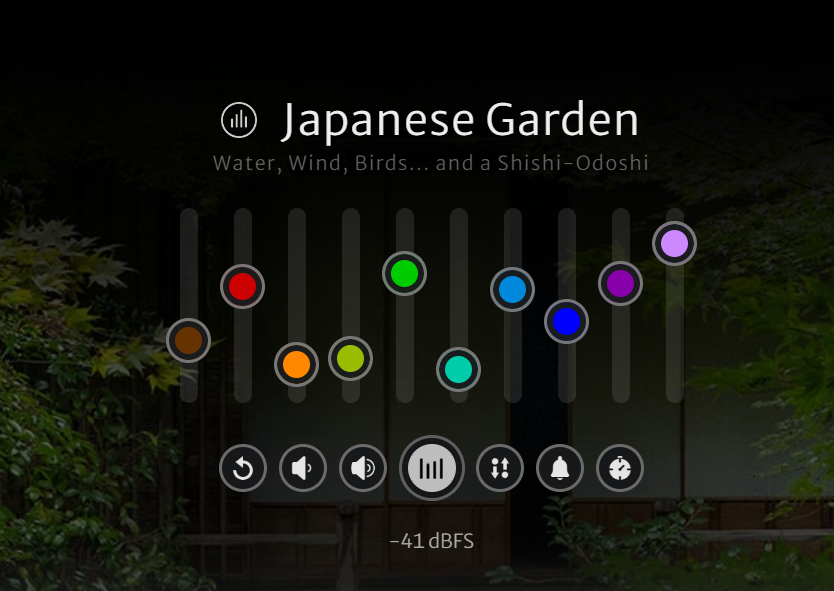
\includegraphics[width=0.5\linewidth]{images/background/mynoise.png}    

    \caption{Screenshot from \textit{mynoise.net}, an ambience generator where users can mix together a number of curated sounds to create a soundscape.}

    \label{fig:mynoise}

\end{figure}

\subsection{Sequencers and Drum Machines}
A sequencer is a common music production tool which typically involves sequencing audio in a loop so that sounds are triggered in a certain pattern. Drum machines are a type of sequencer which are typically limited to short drum or percussion samples, such as kick and snare drums, cymbals, and other percussive sounds like claps or shakers. The main purpose of these is to create drum beats, and there are online tools such as \textit{drumbit.app} (see Figure \ref{fig:drumbit}) or \textit{virtualdrumming.com} which allow for the creation and playback of these patterns. Most tools offer a variety of percussive sounds and typically across 16 time steps, four for each beat in a 4/4 time signature.

\begin{figure}[htb]
    \centering
    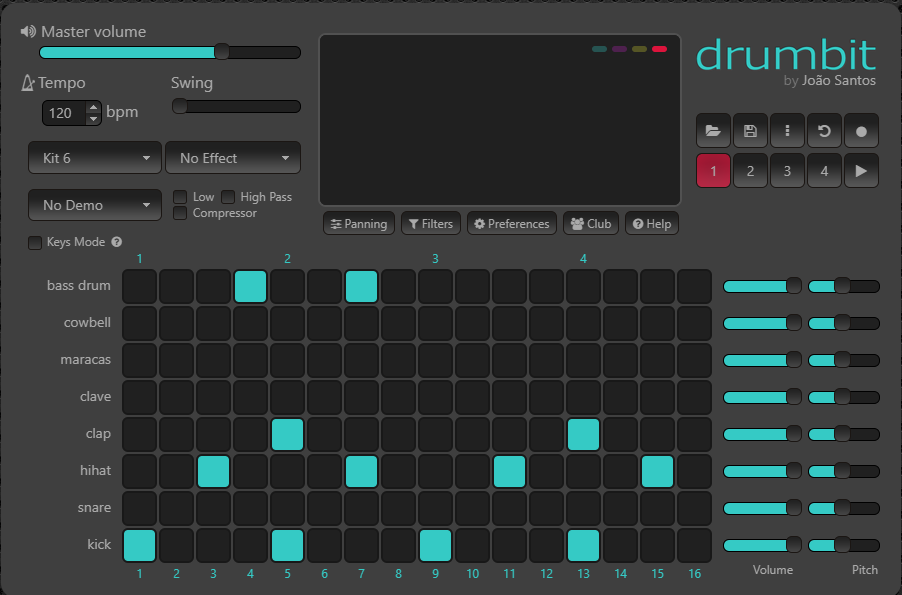
\includegraphics[width=0.5\linewidth]{images/background/drumbit.png}    

    \caption{Screenshot from drumbit.app, a drum machine where users can create a drum pattern by toggling on and off the different drum samples at specified time steps.}

    \label{fig:drumbit}

\end{figure}

Similarly to the ambient sound generators discussed previously, these tools offer plenty of local functionality for their specific purpose (in this case as a drum machine), but do not incorporate instruments or real-time collaboration.

\subsection{Collaborative Music Production and DAWs}
Much of modern music production involves the use of Digital Audio Workstations (DAWs) such as \textit{FLStudio} (see Figure \ref{fig:flstudio}), \textit{Ableton}, or \textit{Reaper}. These applications allow for the recording, editing, and production of music through the use of various methods such as recording live instruments, inputting notes using MIDI controllers, or digitally manipulating sounds using filters and various effects.

\begin{figure}[htb]
    \centering
    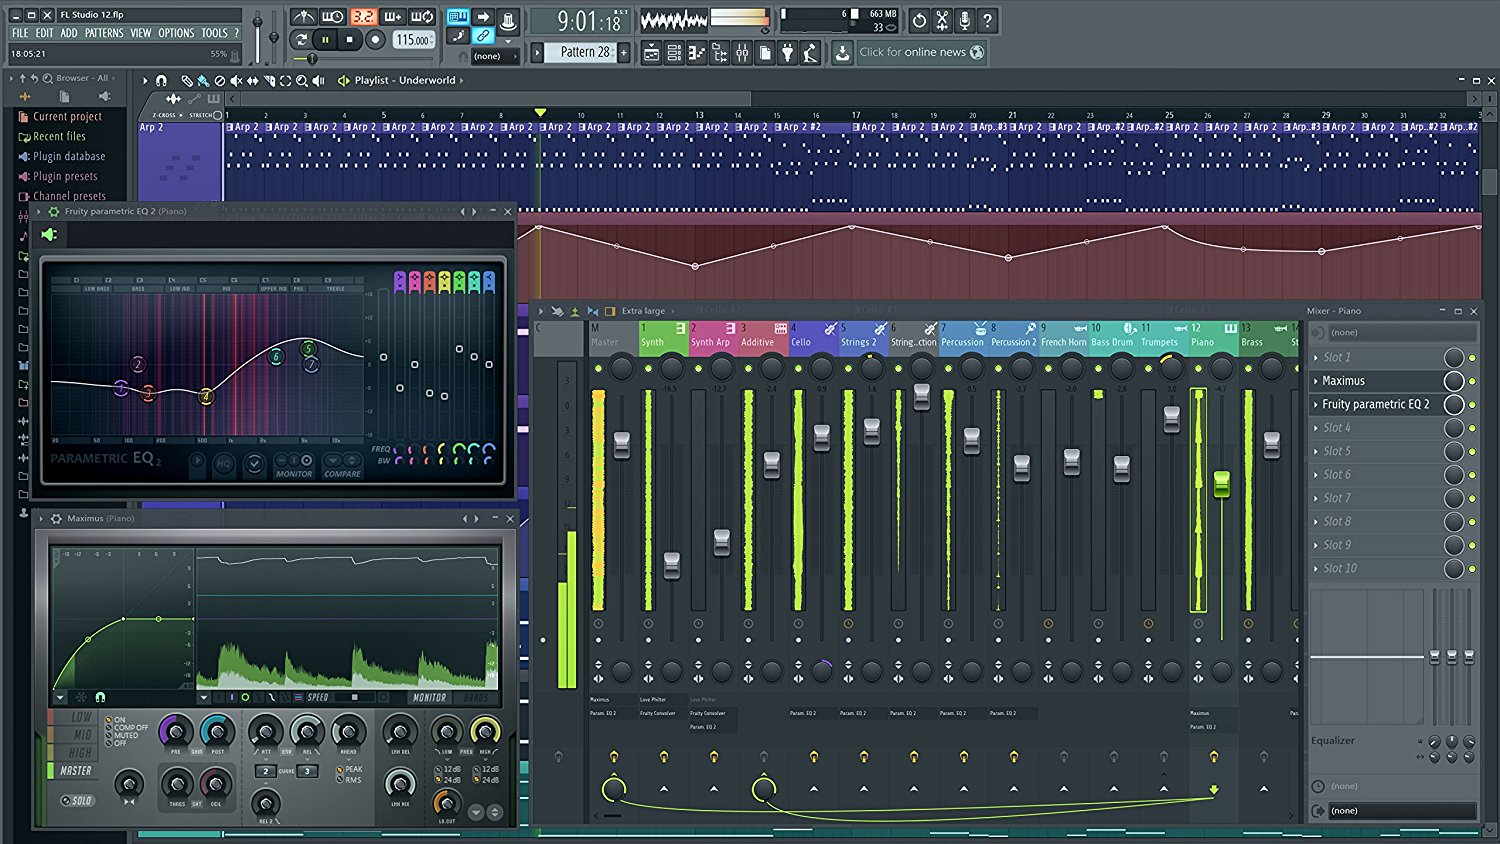
\includegraphics[width=0.5\linewidth]{images/background/flstudio.jpg}    

    \caption{Screenshot from FL Studio, a popular DAW application for producing music.}

    \label{fig:flstudio}

\end{figure}

There are online applications such as \textit{soundtrap.com} (see Figure \ref{fig:soundtrap}), which offer a DAW-like experience through a browser, allowing for collaboration in producing music, however, these tools often require prior music production experience in order to be understood and used effectively. Additionally, the music-making process is usually iterative and finite in nature, as collaboration is done to create a concrete track with a beginning and end. The aim of this project is to create a music-making experience which is accessible for users with no production experience, where music is created in real-time and users can collaborate together to alter how the sound changes as it is being generated.

\begin{figure}[htb]
    \centering
    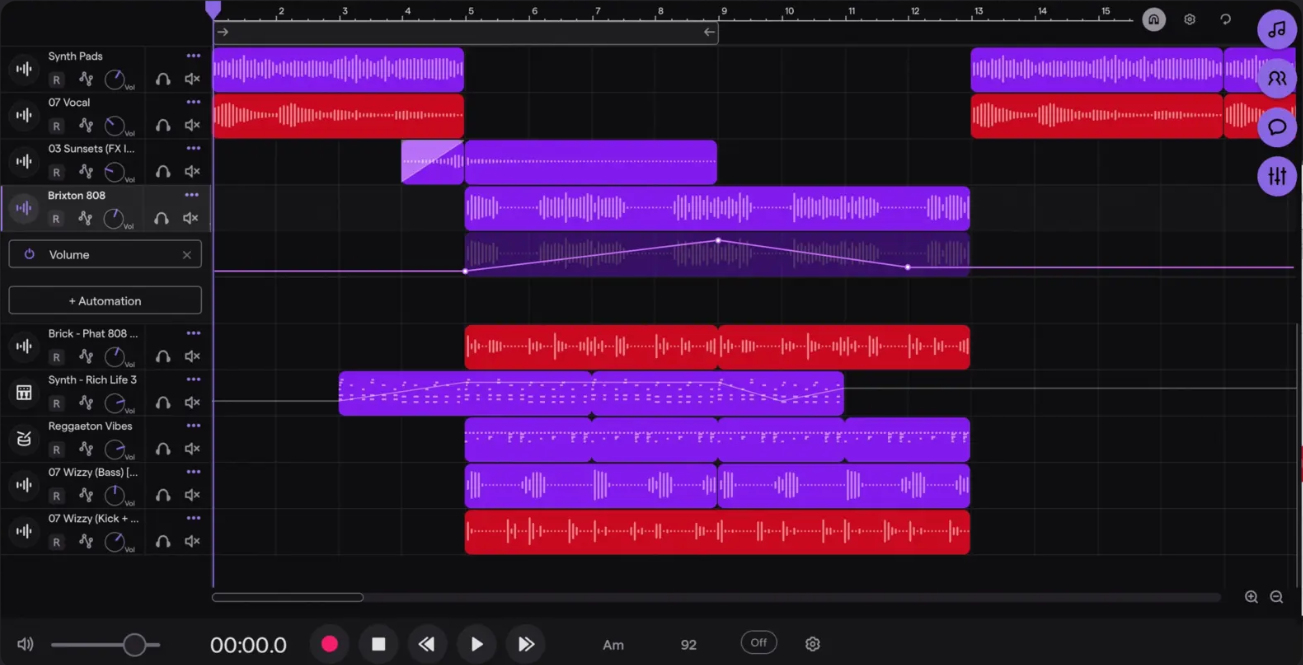
\includegraphics[width=0.5\linewidth]{images/background/soundtrap.png}    

    \caption{Screenshot from soundtrap.com, an online DAW which offers many features as other popular DAWs but in a collaborative online environment.}

    \label{fig:soundtrap}

\end{figure}

\section{Procedurally Generated Music}

Procedurally generated music (sometimes referred to as “adaptive”, “dynamic”, or “interactive” music) generally refers to music which is created algorithmically rather than concretely composed by a person. Typically, this is done through the use of predefined algorithms, parameterisation, and some form of randomisation.

\subsection{Creating Music Algorithmically}
Although randomly generated melodies can be easily achieved by, for example, picking a random piano note every second and playing the result, algorithmically generating convincing music requires a lot more nuisance and a low-level compositional understanding to sound realistic.

A guide for \textit{Procjam} by \cite{procjam} contains information on generating realistic and engaging music by incorporating rules on musical concepts such as repetition, harmonic intervals, and melodic density. Having parameters such as rhythmic density which alter the music generation is a way for users to change the sound as it is being generated.

Commonly found in video games or other interactive entertainment, procedurally generated music can accompany and react in real time to the context or events happening in the game environment. A modern technique called “vertical remixing” is to dynamically swap out instruments to change the musical timbre of the accompanying composition.

\subsection{Implementations}
There are not many online tools which procedurally generate music in real-time. Some sites such as \textit{dopeloop.ai/melody-generator} (see Figure \ref{fig:dopeloop}) or \textit{app.soundgrail.com/melody-generator} offer rudimentary melody creation in various scales, tempos, and instruments, however, neither support real-time generation and playback of those melodies, or allow users to adjust the parameters of the melodies as they are created.

\begin{figure}[htb]
    \centering
    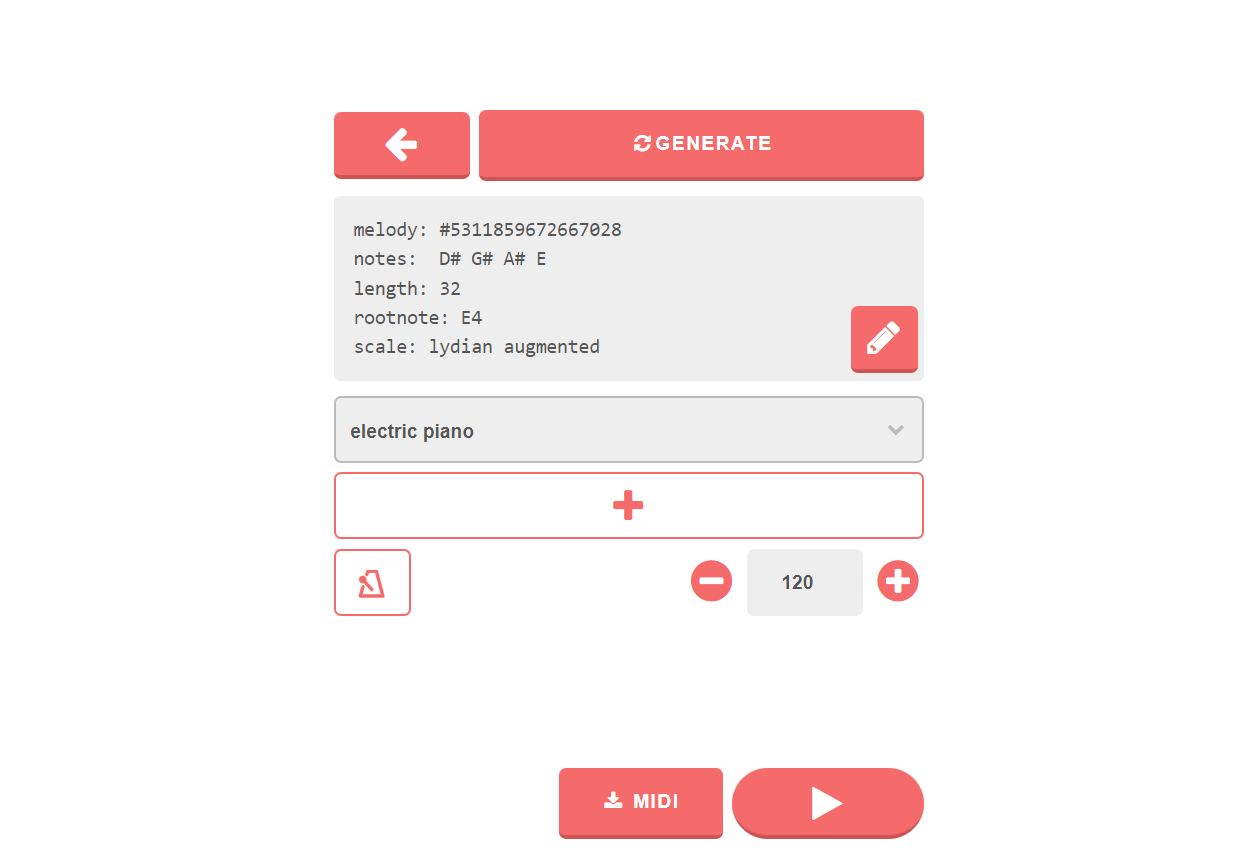
\includegraphics[width=0.5\linewidth]{images/background/dopeloop.png}    

    \caption{Screenshot from dopeloop.ai/melody-generator, a tool to generate and play short melodies in a variety of scales and instruments.}

    \label{fig:dopeloop}

\end{figure}

The design section discusses more on generating music in real-time, in particular the techniques, rules, and algorithms used for this project’s instruments.

\section{Psychology of Collaborative Music-Making}
In traditional collaborative music making, there are strong social and psychological factors which contribute to the result, such as the dynamics between musicians, the effectiveness of communication, and the shared goal of the group. One study by \cite{cunha2012secondary} noted that making music together not only facilitated social and emotional development, but that collaborative music-making developed cognitive skills and was seen as a way to practice and express culture to others.

\section{Consolidating Ideas}
The project will combine aspects and features from each of these categories and consolidate them into one cohesive system which incorporates elements from the categories of music creation covered in this section.


\chapter{Analysis/Requirements}

\section{Analysis}
From background research, it was clear that despite there being many online music creation sites, there were not many applications which played back generated music in real-time and allowed user inputs to change how the music was created as it is generated. There was also a lack of collaborative experiences that were easily accessible to users with little musical experience.

From this, the functional and non-functional requirements can be defined.

\section{Requirements}

\subsection{Functional Requirements}

Site framework:
\begin{itemize}
    \item 
        Users should be able to create an account and login to the app using their credentials.
    \item 
        Users, logged in or not, can join an audio room, and each room should accommodate multiple users to be connected to it.
\end{itemize}

Synchronised functions:
\begin{itemize}
    \item 
        All changes to an audio room should occur in close to real-time.
    \item 
        Users should be able to adjust modifiers or parameters of the different tracks while they are generated and/or are playing.
    \item 
        Users should be able to hear audibly when they change a track’s parameters or modifiers in real time.
    \item 
        Changes made by one user should be reflected to all other connected users with negligible latency.
    \item 
        Each user should hear an identical audio output during a given session.
\end{itemize}

Audio tracks:
\begin{itemize}
    \item 
        There should be three audio tracks, each with its own panel where users can adjust the parameters and modifiers of each track. There will be an ambience mixer, a 16-step sequencer, and a panel with various instruments.
    \item 
        Users should be able to mix several ambient noises together to create a soundscape.
    \item 
        Users should be able to use the sequencer to create a looping drum pattern.
    \item 
        Users should be able to add instruments to the mix and alter how they sound using modifiers and parameters.
\end{itemize}

\subsection{Non-Functional Requirements}

Performance and reliability:
\begin{itemize}
    \item 
        The system should be able to send audio messages consistently and in time with the beat.
    \item 
        The time between a user adjusting a parameter or modifier and that change being synchronised with all other connected users should be minimised.
    \item 
        The system should be able to handle a large number of connected users to a room without significant latency or beat consistency problems.
\end{itemize}

Usability:
\begin{itemize}
    \item 
        The UI should be intuitive and clean so the user is not overwhelmed or confused.
    \item 
        The system should support multiple device sizes and resolutions to provide an accessible and consistent experience across platforms and screen sizes.
\end{itemize}

Deployment:
\begin{itemize}
    \item 
        The app should be fully deployed on a live site with all features working as intended
    \item 
        The deployed app should be stable and live without disruption.
\end{itemize}

Psychosocial:
\begin{itemize}
    \item 
        Users should feel connected to each other while they create music together in an audio room.
    \item 
        Users should feel relaxed and engaged in the music-making process.
\end{itemize}


% Design should cover the abstract design in such a way that someone else might be able to do what you did, 
% but with a different language or library or tool. This might include overall system architecture diagrams,
% user interface designs (wireframes/personas/etc.), protocol specifications, algorithms, data set design choices,
% among others. Specific languages, technical choices, libraries and such like should not usually appear in the design. These are implementation details.

\chapter{Design}

\section{Overview}
The design of the system can be broken down into a few fundamental categories:
\begin{itemize}
    \item 
        The foundational structure of the web app
        \begin{enumerate}
            \item Site structure
            \item Layout of the database
        \end{enumerate}
    \item 
        The three audio tracks which make up the system
        \begin{enumerate}
            \item The ambience mixer
            \item The 16-step sequencer
            \item The various instruments
        \end{enumerate}
    \item 
        The design of the interface
        \begin{enumerate}
            \item Visual design
            \item Sound design
        \end{enumerate}
\end{itemize}
This chapter will cover the key design choices in each of these categories and why they were chosen to fulfil the project’s requirements.

\section{App Foundations}

\subsection{Site Structure}
The site has two main pages plus additional accessory pages for the accounts system and the About page. Most of the site’s functions are on the “Room” pages, where users will interact with the audio systems. The homepage has links to all available rooms, and there are pages on the navigation bar (which is visible sitewide) for signing in, logging out, and registering a new account.

\subsection{Database Layout}
The database for this project is minimal and consists of a Room, Message, and User table.
\begin{itemize}
    \item 
        The Room table has a name and a many-to-many field containing the IDs of the users currently connected to it
    \item 
        The User table contains the username and password of the user alongside other generic information
    \item 
        The Message table contains messages the user has sent into a room and contains the user and room IDs, the content of the message, and the time it was sent
\end{itemize}
Each of the tables uses an auto-incrementing ID field as its primary key. Figure \ref{fig:erd} shows the entity-relationship diagram of the database.

\begin{figure}[htb]
    \centering
    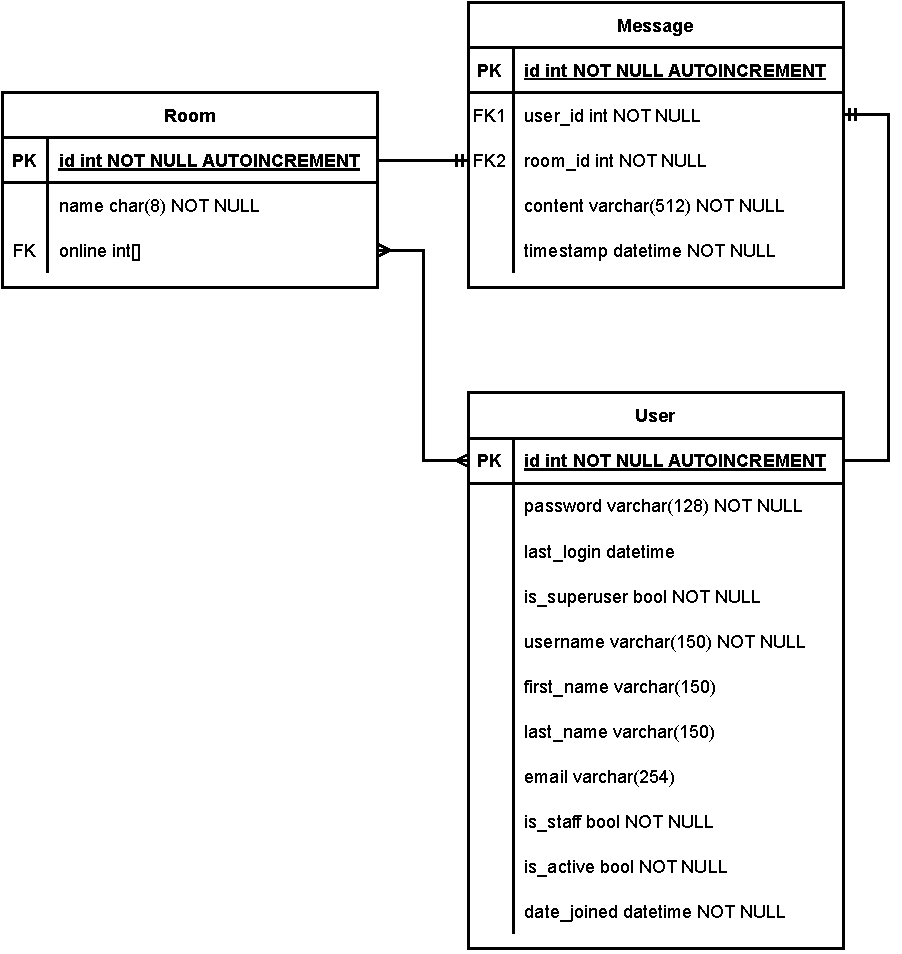
\includegraphics[width=0.5\linewidth]{images/design/entity-relation.pdf}    
    \caption{Entity-relationship diagram of the app's database}
    \label{fig:erd}
\end{figure}

Users register with a username and password. As this site’s user implementation is basic and only used to associate names with chat messages, no other information is required.


\section{Controlling the System}

The room page consists of three main panels, with each corresponding to an audio track. These tracks are:
\begin{itemize}
    \item The ambience mixer
    \item The 16-step sequencer
    \item The various instruments
\end{itemize}

This section will cover the design of each panel, and how certain design decisions were made to meet the requirements specification.

\subsection{Ambience Track}
The ambience panel will consist of a series of sliders which link to the volume of a certain ambient sound. This panel is designed to mimic real-world mixing desks which often include a series of vertical sliders to adjust the gain (volume) of a track. There will also be a mute toggle switch to quickly disable or enable that specific sound. Users will use these sliders to create an ambience mix or soundscape by combining multiple sounds in varying levels. Figure \ref{fig:mixer-design} compares the app's ambience panel to a real-world mixing desk.

\begin{figure}[htb] 
    \centering
    \begin{subfigure}[b]{0.45\textwidth}
        
\includegraphics[width=\textwidth]{images/design/mixing-desk.png}
        \caption{The track sliders of a mixing desk, commonly found in recording studios. (Source: Depositphotos)}
        \label{fig:mixing-desk}
    \end{subfigure}
    ~
    \begin{subfigure}[b]{0.45\textwidth}
        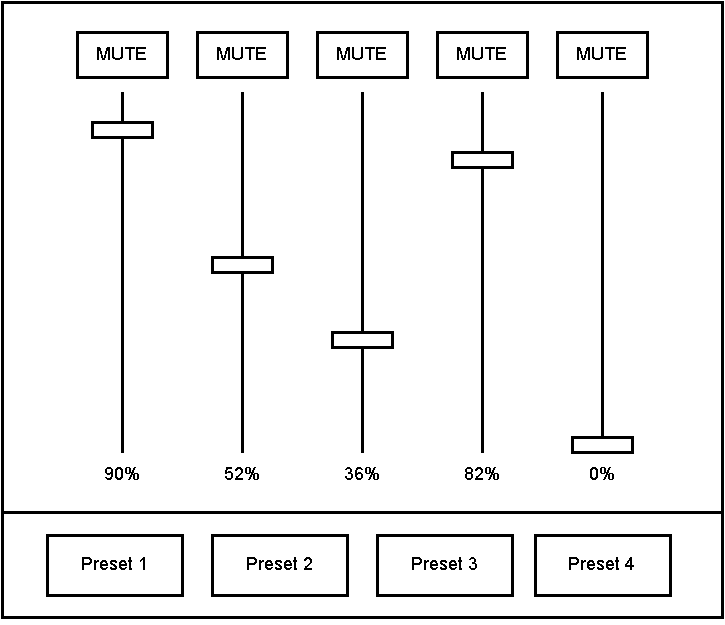
\includegraphics[width=\textwidth]{images/design/mixer-wireframe.pdf}
        \caption{Wireframe of the project's ambience page.}
        \label{fig:mixer-wireframe}
    \end{subfigure}
    ~
    \caption{
    The design of the \subref{fig:mixer-wireframe} ambience page takes after the real-world design of a \subref{fig:mixing-desk} mixing desk.
    }\label{fig:mixer-design}
\end{figure}

The sounds used for each track are similar to sounds available in existing ambient generator sites, for example, heavy thunder, a crackling fire, a recording of a coffee shop, and crickets chirping. These sounds were chosen because

In addition, there will be preset soundscapes which users can click on to slide the mixer to a pre-defined state. This is also similar to real-world mixing desks, where user-defined states can be saved and loaded, triggering the physical sliders to smoothly slide to that state. The mixer should emulate that sliding animation so that the transition between presets looks more realistic and natural, which benefits the user experience.

\subsection{Sequencer Track}
The sequencer panel primarily consists of a grid of buttons which represent the 16 timesteps across 8 different drum samples. When the buttons are clicked, they will light up to indicate that they are enabled. As the sequencer loops one column at a time through the timesteps from left to right (or steps 0 to 15), they will play any enabled sample at that given timestep. For example, in Figure \ref{fig:sequencer-wireframe}, in step 3, the sequencer will play the “Closed Hi-Hat” and “Crunch” samples, while in step 12, the “Kick” and “Snare” samples will play. Once the sequence reaches step 15, it resets back to step 0 and traverses the steps again. This is similar to existing implementations of online drum machines as well as real-world step sequencers.

\begin{figure}[htb]
    \centering
    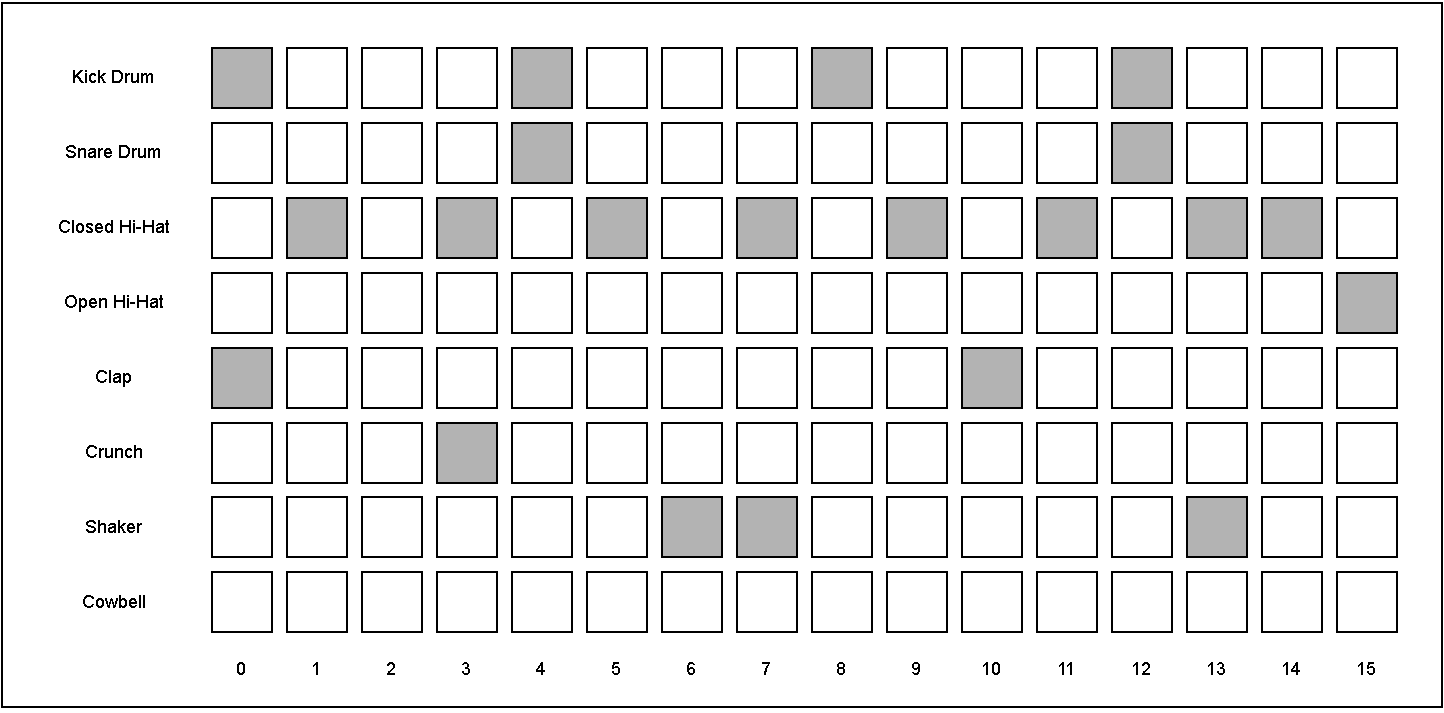
\includegraphics[width=0.8\linewidth]{images/design/sequencer-wireframe.pdf}    
    \caption{Wireframe of the project's sequencer page.}
    \label{fig:sequencer-wireframe}
\end{figure}

The chosen samples are popular percussion sounds and are commonly found in similar systems, such as kick and snare drums, cymbals, and claps. Additionally, the individual tracks will be able to be muted/unmuted to quickly turn on and off specific samples. There should also be a button to clear the sequencer, which turns off all active buttons.


\subsection{Instrument Track}
The instrument panel contains the different instruments that can be added to the mix, and their modifiers and parameters. Initially, this page was designed to use circular knobs to adjust the parameters as this more closely mimicked real-world controls, for example, the volume and tone knobs on an electric guitar (see Figure \ref{fig:guitar-knobs}). However, when testing these with a mouse it was more difficult to precisely control the levels of the parameters compared to the sliders used in the previous two panels. It also required a lot more custom scripting and event listeners compared to sliders, which are a built-in HTML element.

\begin{figure}[htb]
    \centering
    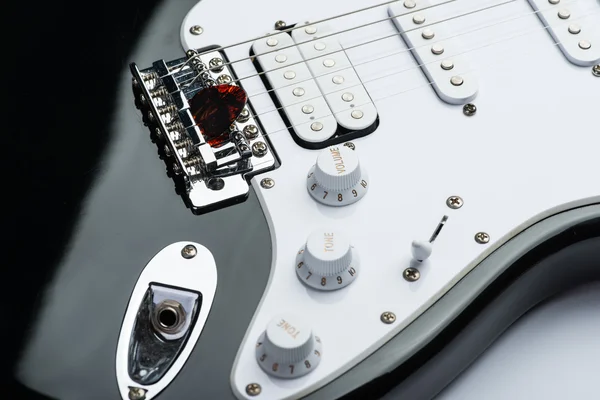
\includegraphics[width=0.5\linewidth]{images/design/guitar-knobs.png}    
    \caption{Electric guitars typically use twistable knobs to control their volume and tone (Source: Depositphotos).}
    \label{fig:guitar-knobs}
\end{figure}

Instead, sliders are used to adjust the parameters and modifiers of their corresponding instrument. Although this was not as aesthetically pleasing as using control knobs, it was more user-friendly and accessible for smaller devices due to the larger control surface enabling more precise adjustments. See the comparison between the two designs in Figure \ref{fig:instrument-wireframe}.

\begin{figure}[htb] 
    \centering
    \begin{subfigure}[b]{0.45\textwidth}
        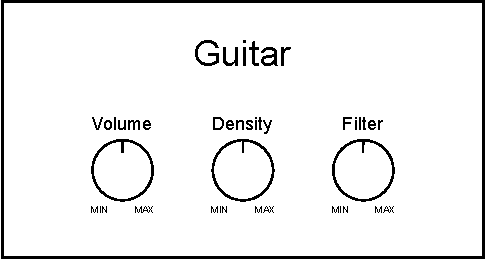
\includegraphics[width=\textwidth]{images/design/instrument-knob-wireframe.pdf}
        \caption{Wireframe of an instrument box using knobs.}
        \label{fig:instrument-knob-wireframe}
    \end{subfigure}
    ~
    \begin{subfigure}[b]{0.45\textwidth}
        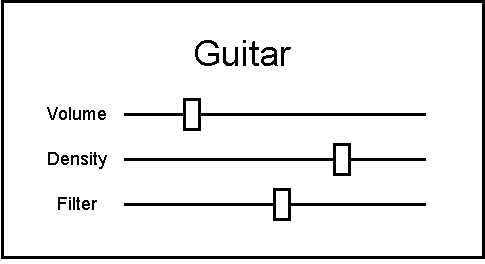
\includegraphics[width=\textwidth]{images/design/instrument-slider-wireframe.pdf}
        \caption{Wireframe of an instrument box using sliders.}
        \label{fig:instrument-slider-wireframe}
    \end{subfigure}
    ~
    \caption{
    Compared to \subref{fig:instrument-knob-wireframe} knobs, \subref{fig:instrument-slider-wireframe} sliders offer a larger control surface area.
    }\label{fig:instrument-wireframe}
\end{figure}

Each instrument will uniquely generate its part in real time, allowing users to adjust their parameters as the instrument plays. The instruments will be balanced so that they support each other compositionally, for example, some instruments will have the role of supporting the mix rhythmically by playing more steadily in an accompaniment style, while other instruments will have more of a lead role, generating melodies on top of the existing instrumentation.

According to the requirements specification, users should have sufficient control over the instruments so they feel like they are contributing significantly to the overall sound of a given session. There are two types of modifiers which will be used in this system: Filters, which modify the timbre or tone of the output sound, and generator parameters, which will change how the instruments pick which notes to play and when they play them. As the instruments play, the user can adjust their volume and any instrument-specific parameters. The implementation section will cover which instruments were added, and the behaviour of each.

All the instruments follow a similar behaviour, with the one exception of the guitar. Instead of picking a note or notes to play at a given timestep, the guitar is pre-programmed with a concrete set of MIDI recordings lasting two measures/bars of music each, where each phrase has an associated “intensity” and “density” label. For example, if the user sets the intensity to “medium” and the density to “sparse”, the guitar will randomly pick a pre-recorded phrase which is labelled with medium intensity and sparse density, playing that sample at the start of the next two measures.

The guitar is defined this way to allow for greater expressive control over the instrument, allowing pitch bends, vibrato, and more complex rhythmic phrasing to be included in the samples, which would not be possible if the guitar used the same system as the other instruments.

\subsection{Integrating Tracks}
The three audio tracks are designed to integrate seamlessly and harmoniously to create a cohesive and continuous musical composition. The ambience track plays continuously, with the sounds perpetually looping to create an auditory backdrop to the sound mix. The sequencer and instrument tracks are triggered simultaneously and follow a pulse which is sent from the server to each client, allowing the drums to play perfectly in time with the instruments.


\section{Interface Design}

\subsection{Navigation between Panels}
To navigate between the three track panels, there will be a navigation bar. When the page loads, the panels will be hidden apart from the ambience panel which is open by default. Then, when the user clicks on a panel the current panel will fade out while the new panel fades in. The room page will use this layout to simplify the appearance of the app and not overwhelm the user with options and controls. Additionally, one panel is visible at a time on purpose so that when multiple users are using the system, one user can be controlling one panel while another user can be controlling a separate panel. This should encourage collaboration since a user can only control one track at a given time.

The navigation bar (Figure \ref{fig:navigation-wireframe}) also doubles as a master mixer, as there will be volume sliders which control the master volume for its associated track.

\begin{figure}[htb]
    \centering
    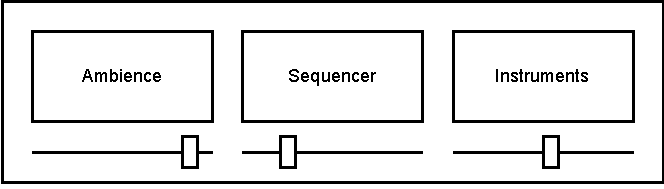
\includegraphics[width=0.5\linewidth]{images/design/navigation-wireframe.pdf}    
    \caption{Wireframe for the navigation bar with master volume sliders underneath each track.}
    \label{fig:navigation-wireframe}
\end{figure}

\subsection{Visual Design}
As mentioned previously, much of the design purposely mimics existing real-world technologies and systems, such as mixing desk sliders and step sequencer button grids. Known as “Skeuomorphism”, this design style has been proven in a study by \cite{urbano2022skeuomorphism} to be more effective and accurate at conveying interface elements which can be clicked or interacted with when compared to more flat or minimalist designs. Skeuomorphism is commonplace amongst music production software, an example of which can be seen with audio compressor plugins in Figure \ref{fig:compressor}.

In addition to using skeuomorphic-inspired design, adding visual cues like changing the colour or size of interface elements when users hover their mouse cursor over them also helps to indicate when an element can be interacted with, so these cues will be in place for all of the interactable controls in the system.

\begin{figure}[htb] 
    \centering
    \begin{subfigure}[b]{0.45\textwidth}
        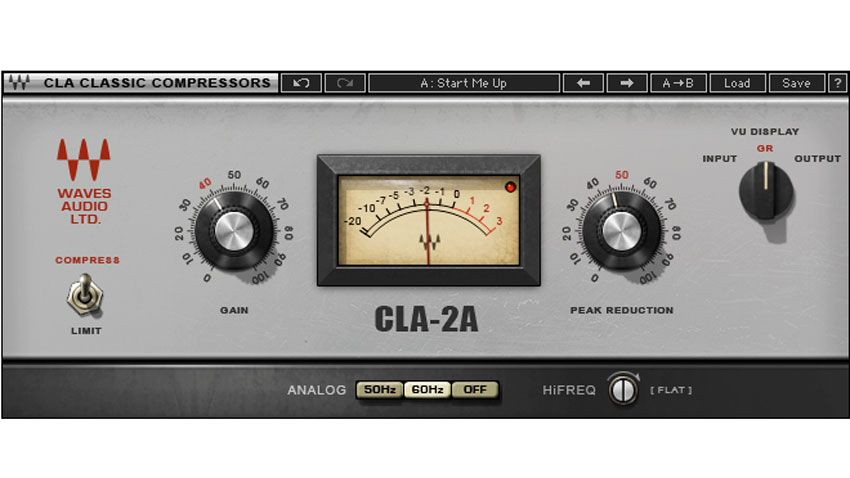
\includegraphics[width=\textwidth]{images/design/compressor-digital.png}
        \caption{A digital compressor plugin for a DAW. (Source: Waves Audio)}
        \label{fig:compressor-digital}
    \end{subfigure}
    ~
    \begin{subfigure}[b]{0.45\textwidth}
        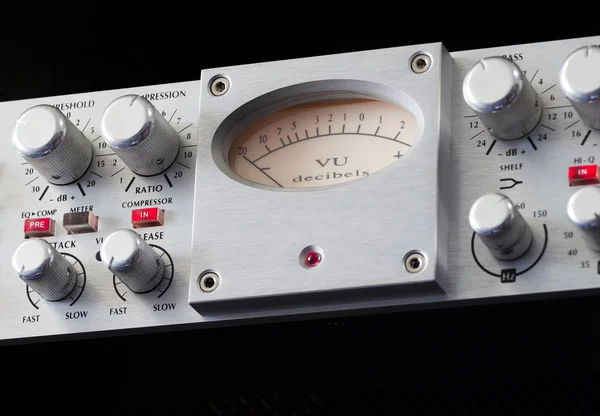
\includegraphics[width=\textwidth]{images/design/compressor-analogue.png}
        \caption{A physical analogue compressor. (Source: Depositphotos)}
        \label{fig:compressor-analogue}
    \end{subfigure}
    ~
    \caption{
    Digital music production plugins like \subref{fig:compressor-digital} often mimic the look and feel of physical analogue units like \subref{fig:compressor-analogue}. 
    }\label{fig:compressor}
\end{figure}

\subsection{Sound Design}
In addition to the system’s visual design. The user experience can be positively affected by the sound design of the app. Providing immediate auditory feedback confirms that their action has been recognised by the system and helps build their confidence in interacting with the interface. It has also been proven to help reduce cognitive load as users can rely on auditory cues to confirm their actions. One particular study by \cite{jeon2015menu} found that adding auditory cues to a car’s infotainment system resulted in a lower perceived workload when executing tasks such as scrolling through music playlists. This allowed drivers to operate menus more efficiently while driving more safely. This is important to create a relaxing atmosphere and immerse the user as they can pay more attention to the music-making experience.

Some examples of these cues are button-pressing sounds when the user clicks on a toggle switch, or notch sounds when the user interacts with a slider control. Similarly to the visual design, these sounds will be chosen to mimic real-world interactions with controls such as buttons, switches, and mixer sliders. A study by \cite{sikora1995musical} found that real-world sounds mapped more reliably and predictably to corresponding GUI functions compared to more abstract auditory cues. Therefore, by incorporating real-world sounds into the interface, the system’s design can leverage users’ existing mental models, making it easier for them to interpret the auditory feedback.


\lstdefinelanguage[ECMAScript2015]{JavaScript}[]{JavaScript}{
  morekeywords=[1]{await, async, case, catch, class, const, default, do,
    enum, export, extends, finally, from, implements, import, instanceof,
    let, static, super, switch, throw, try},
  morestring=[b]` % Interpolation strings.
}
\lstalias[]{ES6}[ECMAScript2015]{JavaScript}


\chapter{Implementation}
% What did you do to implement this idea, and what technical achievements did you make?
% You can't talk about everything. Cover the high level first, then cover important, relevant or impressive details.

This chapter will cover the implementation details of the project, including the technologies used to develop the system, the unique and/or novel technical features of the app, and the deployment of the project onto a live website.

\section{Chosen Technologies}

\subsection{Web Framework}
The project was designed to be made as a web app from the very beginning. There are several advantages and drawbacks but ultimately this was the preferred platform to develop the project on. A web app would be the most accessible way for users to quickly access the project as no installation is required. Additionally, the project would be inherently cross-platform and viewable on a large variety of devices, further increasing the accessibility and ease of use, which was a priority.

Naturally, developing a complex application using web technologies had its drawbacks such as performance concerns. From prior experience, web apps have often required a focus on optimisation and a careful balance between practicality and seamlessness. Since there would be many audio assets which the end user would be required to download, it was important to take into account users with slower internet connections when designing the app. Furthermore, due to the many possible aspect ratios, resolutions, and physical screen sizes that a browser can be used in, the design had to be responsive and work seamlessly with as many different browsers and sizes as possible. The implementation chapter discusses the technical aspects and considerations to achieve the previously defined usability requirements.

The chosen framework would need to support real-time, asynchronous, event-driven communication between the web server and any connected clients. This is because to synchronise the auditory experience to be identical across all connected users, especially while any of the users can make changes to the modifiers or parameters of the music generation, clients would need to send regular state updates to the server. Then, the server can pass on these update events to any other connected client so that they can reflect the same change locally so that each user hears the same audio output at the same time.

The obvious choice for this was to use the WebSockets protocol to provide this two-way communication between the server and clients (See Figure \ref{fig:websocket}). This would have minimal latency and allow for efficient, close-to-real-time updates since messages could be sent through the socket without continuous polling requests from the client over HTTP. The server could also send messages to all connected clients to, for example, ensure a consistent rhythmic beat or pulse.

\begin{figure}[htb]
    \centering
    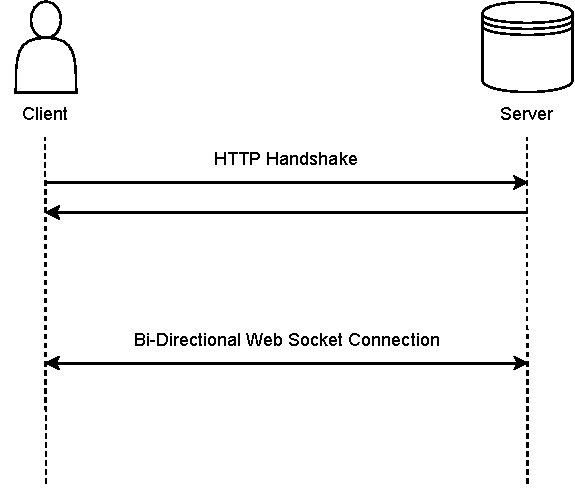
\includegraphics[width=0.5\linewidth]{images/implementation/websocket.pdf}    
    \caption{The WebSocket API provides a bi-directional connection between a client and server, enabling full-duplex communications between the two.}
    \label{fig:websocket}
\end{figure}

A suitable web framework which was ultimately chosen for the project was Django with the Channels extension, which adds support for the WebSockets API. Additionally, with Django offering easy-to-use ORM and templating tools, it was the clear choice for rapid development.

The server sends socket messages through Django Channel’s “Consumer” model, while on the client-side, local JavaScript functions are in charge of receiving, parsing, and sending messages through the socket.


\subsection{Integrating Audio}
After choosing the right web framework, the second most important technology decision was choosing a system to integrate audio into the app, as serving audio in a timely and efficient manner was paramount to the user experience.

The Web Audio API is a relatively new technology, with its release as a W3C recommendation in 2021. It provides a system for loading, processing, and synthesising audio within web applications and offers a high degree of flexibility and modularity. For this project, it was another obvious choice as it is currently the only JavaScript API which supports modular routing, allowing for audio to be manipulated in a number of ways while it is being played.

To do this, audio in the Web Audio API occurs inside of an audio context, where source nodes convey an audio source such as an instrument sample mp3 file. Various audio nodes can then be attached to this source before finally connecting to the context’s destination, for example, the user’s headphones. These audio nodes include gain nodes which allow the volume of the source to be adjusted, and filter nodes which can apply a frequency cutoff to the source, i.e. a low or high-pass filter. Figure \ref{fig:web-audio-api} illustrates a simplified workflow for establishing, manipulating, and outputting an audio source.

By linking frontend controls such as sliders or buttons to functions which modify these audio node properties, users can modify the sound of an audio source as it is being played. Utilising this dynamic node system is crucial for this project to succeed as the requirements specify that users should have control over the sounds as they are being played and/or generated.

\begin{figure}[htb]
    \centering
    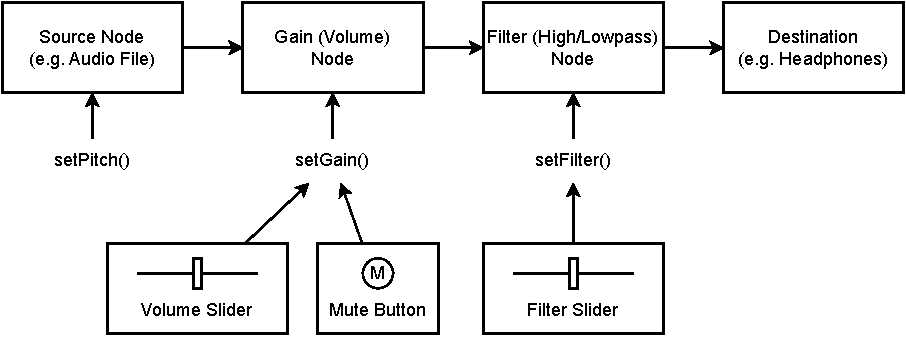
\includegraphics[width=0.7\linewidth]{images/implementation/web-audio-api.pdf}    
    \caption{A simplified audio node diagram, where an audio source is created, then connected to two modifier audio nodes before reaching the context's destination. The setGain() and setFilter() functions are examples of how the interface controls can actively manipulate the sound of a given source (e.g. an instrument sample, ambient sound file, etc.).}
    \label{fig:web-audio-api}
\end{figure}

\subsection{Interface Design}
The interface will be styled using fully custom stylesheets as there is total control over every element of the interface compared to using CSS libraries such as Tailwind or Bootstrap. Although this will increase the implementation time due to styling every element manually, the project’s focus is on creating an engaging and immersive user experience. Decisions which benefit the user experience such as increased control over the site’s appearance are worth the additional time and complexity.

For interactive elements like control surfaces and dynamic visual aspects, local JavaScript scripts will be used alongside jQuery to simplify development.


\section{The Audio System}
The audio system is one of the more novel aspects of this project. Using the Web Audio API to load, manipulate, and deliver sound to the user required many attempts and revisions to get working reliably and consistently. This section will cover some of the technical aspects of creating the musical experience.

\subsection{Tracks and Nodes}
The audio system is comprised of four tracks:
\begin{enumerate}
    \item An ambience track for the ambient mix
    \item A sequencer track for the drum machine
    \item An instrument track for playing the various instruments
    \item A UI track for triggering auditory cues when users interact with controls
\end{enumerate}

Each track is an object which has several audio sources, where each source has a source node, a gain node, and a filter node. Prototype methods are used to manipulate these nodes and UI controls use event listeners to link them to these methods.

For example, the ambience track has seven audio sources which depict the seven ambient sounds users can mix together. Each of these sources has its own gain and filter nodes, allowing each sound to be independently controlled. When a user drags a volume slider, an event listener sees this input and triggers an associated \verb|setGain()| function for whichever sound the slider was associated with. Additionally, this event listener sends a message through the socket so the server can forward the volume update to any other connected users, which then parse this message and update their own gain nodes. See Figure \ref{fig:socket} for an illustration of this example. More information on the socket messages is described later in this chapter.

\begin{figure}[htb]
    \centering
    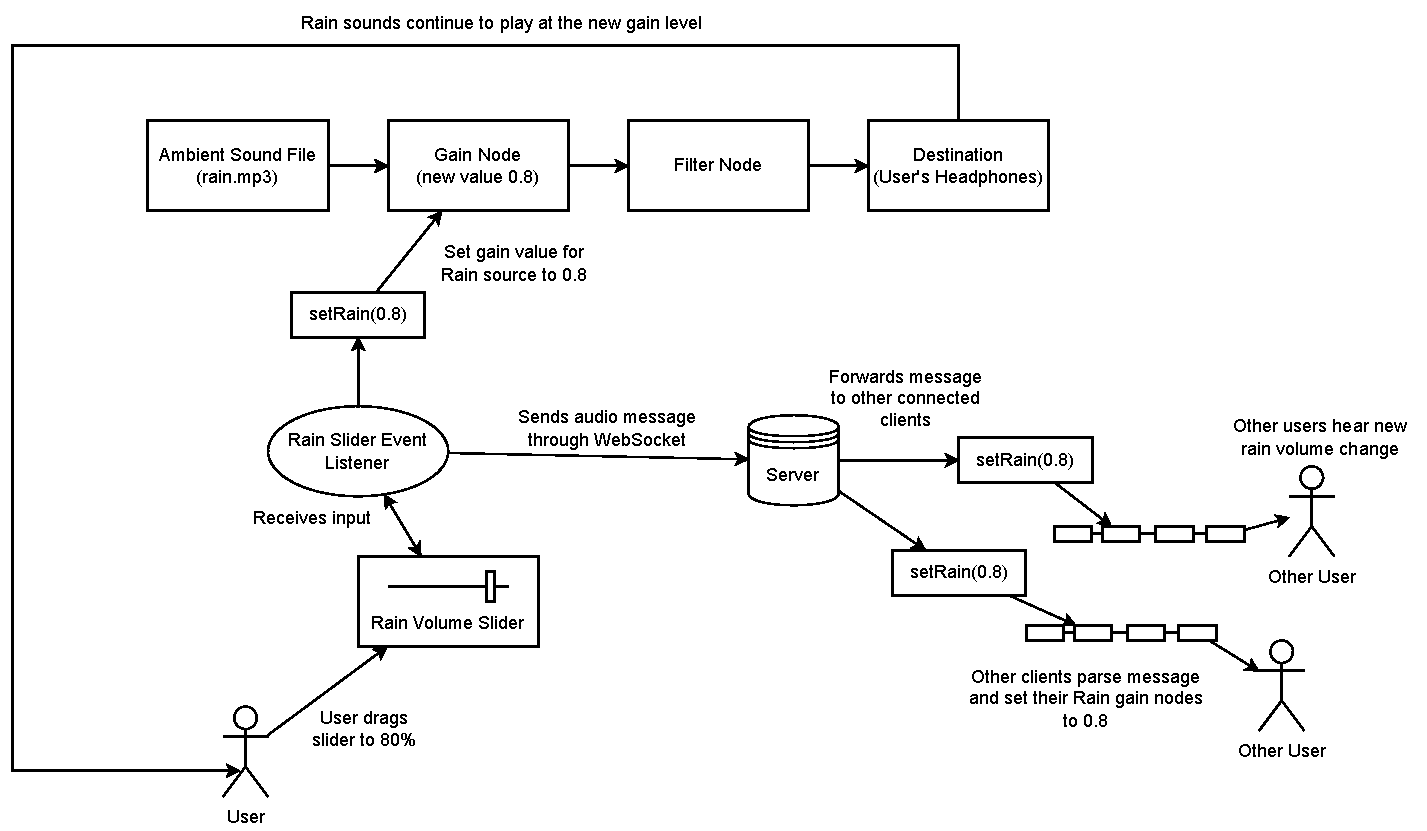
\includegraphics[width=0.8\linewidth]{images/implementation/socket.pdf}    
    \caption{An example of a user interacting with the "Rain" volume slider and how this not only adjusts their own local gain but every other connected user's Rain sample gain as well.}
    \label{fig:socket}
\end{figure}

Each track has its own methods to serve its specific purposes, but all tracks have sources which consist of a similar audio node structure. Instruments, for example, generally have a source node which contains a recording of that instrument playing one note. To create music, however, the instruments need to be able to play lots of different notes.

\subsection{Manipulating Pitch}
To play different notes, a sample is pitch-shifted by either increasing or decreasing its playback speed. All of the instruments apart from the guitar are a single mp3 file of that instrument playing a note at 440Hz, or “A4” in Scientific Pitch Notation (where A is the note and 4 is the octave). By doubling or halving the frequency, the output is the same note in a higher or lower octave. In an octave, there are 12 semitones (i.e. A3 and A4 are 12 notes apart). See Figure \ref{fig:keyboard} for an illustration of this.

\begin{figure}[htb]
    \centering
    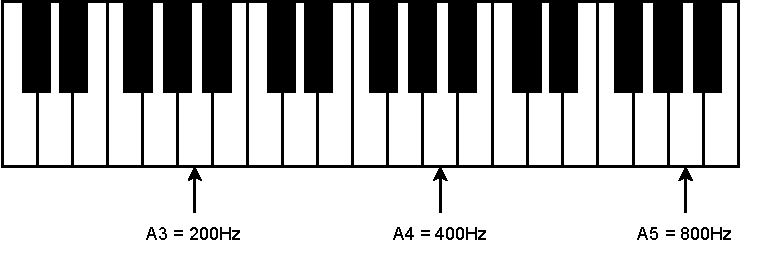
\includegraphics[width=0.7\linewidth]{images/implementation/keyboard.pdf}    
    \caption{A piano keyboard with labels for the A3, A4, and A5 notes.}
    \label{fig:keyboard}
\end{figure}

Audio source nodes in the Web Audio API have a property called “detune”, which offsets the playback frequency by cents. In music, a cent is one-hundredth of a semitone, so setting the detune property to +100 would sound the sample at one semitone higher, and a value of -100 would sound the sample at one semitone lower in pitch. Using this information, a map can be created which maps notes to their corresponding detune value. For example, A4 would be +0, B4 would be +200, F4 would map to -400, etc.

The JavaScript code in Listing \ref{lst:offsets} creates a map between notes in Scientific Pitch Notation to the detune value in cents required to pitch a sample playing at 440Hz to that note.

\begin{lstlisting}[float, caption={Creates a map "noteCentsOffsets" between notes in Scientific Pitch Notation to the detune value in cents required to pitch a sample playing at 440Hz to that note}, label=lst:offsets]

    // Generate equal temperament notes list
    const range = (start, stop) => Array(stop - start + 1).fill().map((_, i) => start + i);
    const octaveRange = range(0, 8).map(val => [val, val - 4]);
    const semitoneOffsets = [
        ["C", -9], ["C#", -8], ["Db", -8], ["D", -7], ["D#", -6], ["Eb", -6], ["E", -5], ["F", -4],
        ["F#", -3], ["Gb", -3], ["G", -2], ["G#", -1], ["Ab", -1], ["A", 0], ["A#", 1], ["Bb", 1], ["B", 2],
    ];
    const notes = octaveRange.reduce((ob, [range, multiplier]) => semitoneOffsets.reduce((ob, [note, semitones]) => ({
        ...ob,
        [note + range]: 440 * Math.pow(2, (semitones + (multiplier * 12)) / 12),
    }), ob), {});
    
    
    // Map each note to its offset in cents (100 cents p/ semitone) relative to 440 Hz
    const noteCentsOffsets = {};
    Object.keys(notes).forEach(note => {
      const frequency = notes[note];
      const centsOffset = 1200 * Math.log2(frequency / 440);
      noteCentsOffsets[note] = centsOffset;
    });

\end{lstlisting}

After this, the instrument’s \verb|sound()| method can take in a note parameter, and then offset the source node of the specified sample by looking up the note in the offsets mapping. For example, \verb|instrumentTrack.sound(“piano”, “C6”)| would create a new source using the \verb|piano.mp3| file, detune it by +1500 cents, and then play it. This is how instruments can play different notes with only one audio sample, and by creating pitches this way, fewer audio files are required to be loaded by clients, lowering the network requirement for users to use the app and therefore increasing its accessibility.

\subsection{Harmonising Instruments}
In music, two notes can sound generally either sound “consonant/harmonious” or “dissonant”, where the former typically sounds more pleasing. Notes can sound dissonant when the ratio between their respective frequencies is farther from being an integer. For example, the notes C and G sound consonant because their frequency ratio is 3:2, while the notes F and B have a frequency ratio of 64:45, and subsequently these notes sound dissonant and generally unpleasing when played together.

In this project, instruments are limited to playing notes in the G flat major pentatonic scale. The pentatonic scale is unique because all of the notes in the scale sound consonant with all the other notes, meaning no matter what combination is playing, there will not be any unpleasing dissonance. This means that the instruments will never clash harmonically and can be programmed to play (essentially) random notes so long as they are in the correct scale.

Harmony, however, is not the only aspect of creating music which is perceived as cohesive and/or natural. The instruments need to play in complementary styles and in a way which sounds organic.

\subsection{Generating Organic-Sounding Music}
Each instrument follows a set of pre-defined rules which were set to make them sound natural and human-like. The most comprehensive example is the piano part, which this section will describe.

First, a random number is generated with a minimum value of zero, and a maximum value of 6-26, which is set by the user using the “density” slider. Then, a switch statement will attempt to match that number to a pre-defined variation.

\begin{itemize}
    \item If the number is 0, the piano generates a chord comprised of three notes
    \item If 1, the piano plays a smaller chord comprised of two notes
    \item If 2 or 3, a single note is played
    \item If 4, the piano plays two notes in succession
    \item If 5, a triplet is played (three notes in succession)
\end{itemize}

If the number does not match any of the cases, then the piano will play nothing. A new number is generated every half-beat, which means eight numbers will be generated and matched to a variation through the course of one bar of music.

When compared to a more rudimentary method of generating melodies, for example by choosing a random note for every beat and then playing it, these rules generate a piano part which sounds more organic and musically purposeful. Figure \ref{fig:piano} compares the notation of an excerpt of the piano’s algorithm with a high density with one that generates a random note for every beat.

\begin{figure}[htb] 
    \centering
    \begin{subfigure}[b]{0.45\textwidth}
        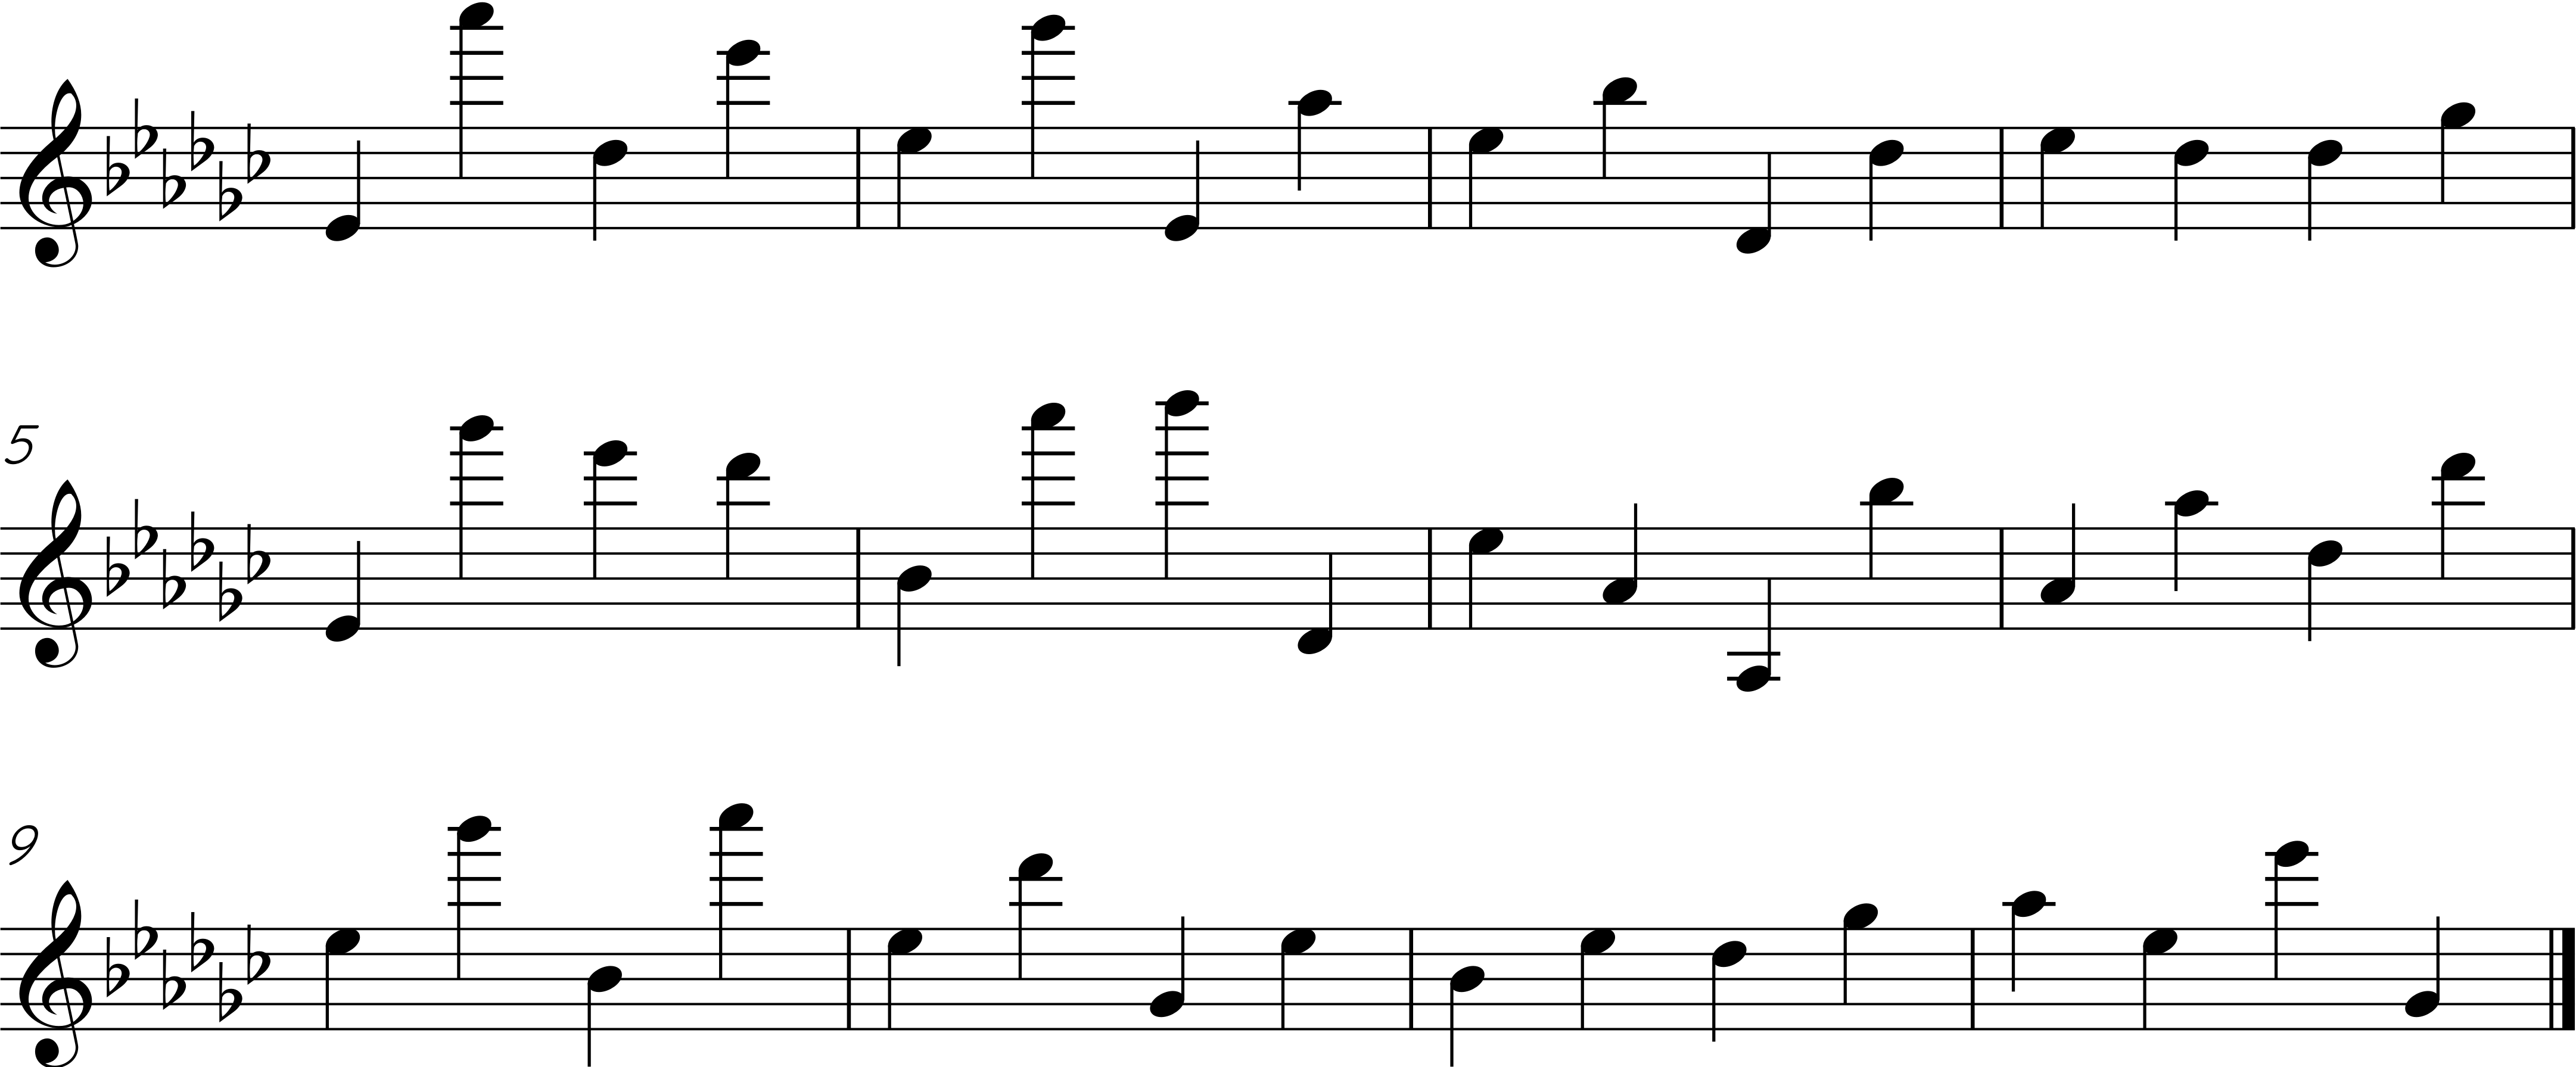
\includegraphics[width=\textwidth]{images/implementation/generated-piano-basic.png}
        \caption{A basic algorithm for generating a melody by choosing a random note of the scale every beat.}
        \label{fig:generated-piano-basic}
    \end{subfigure}
    ~
    \begin{subfigure}[b]{0.45\textwidth}
        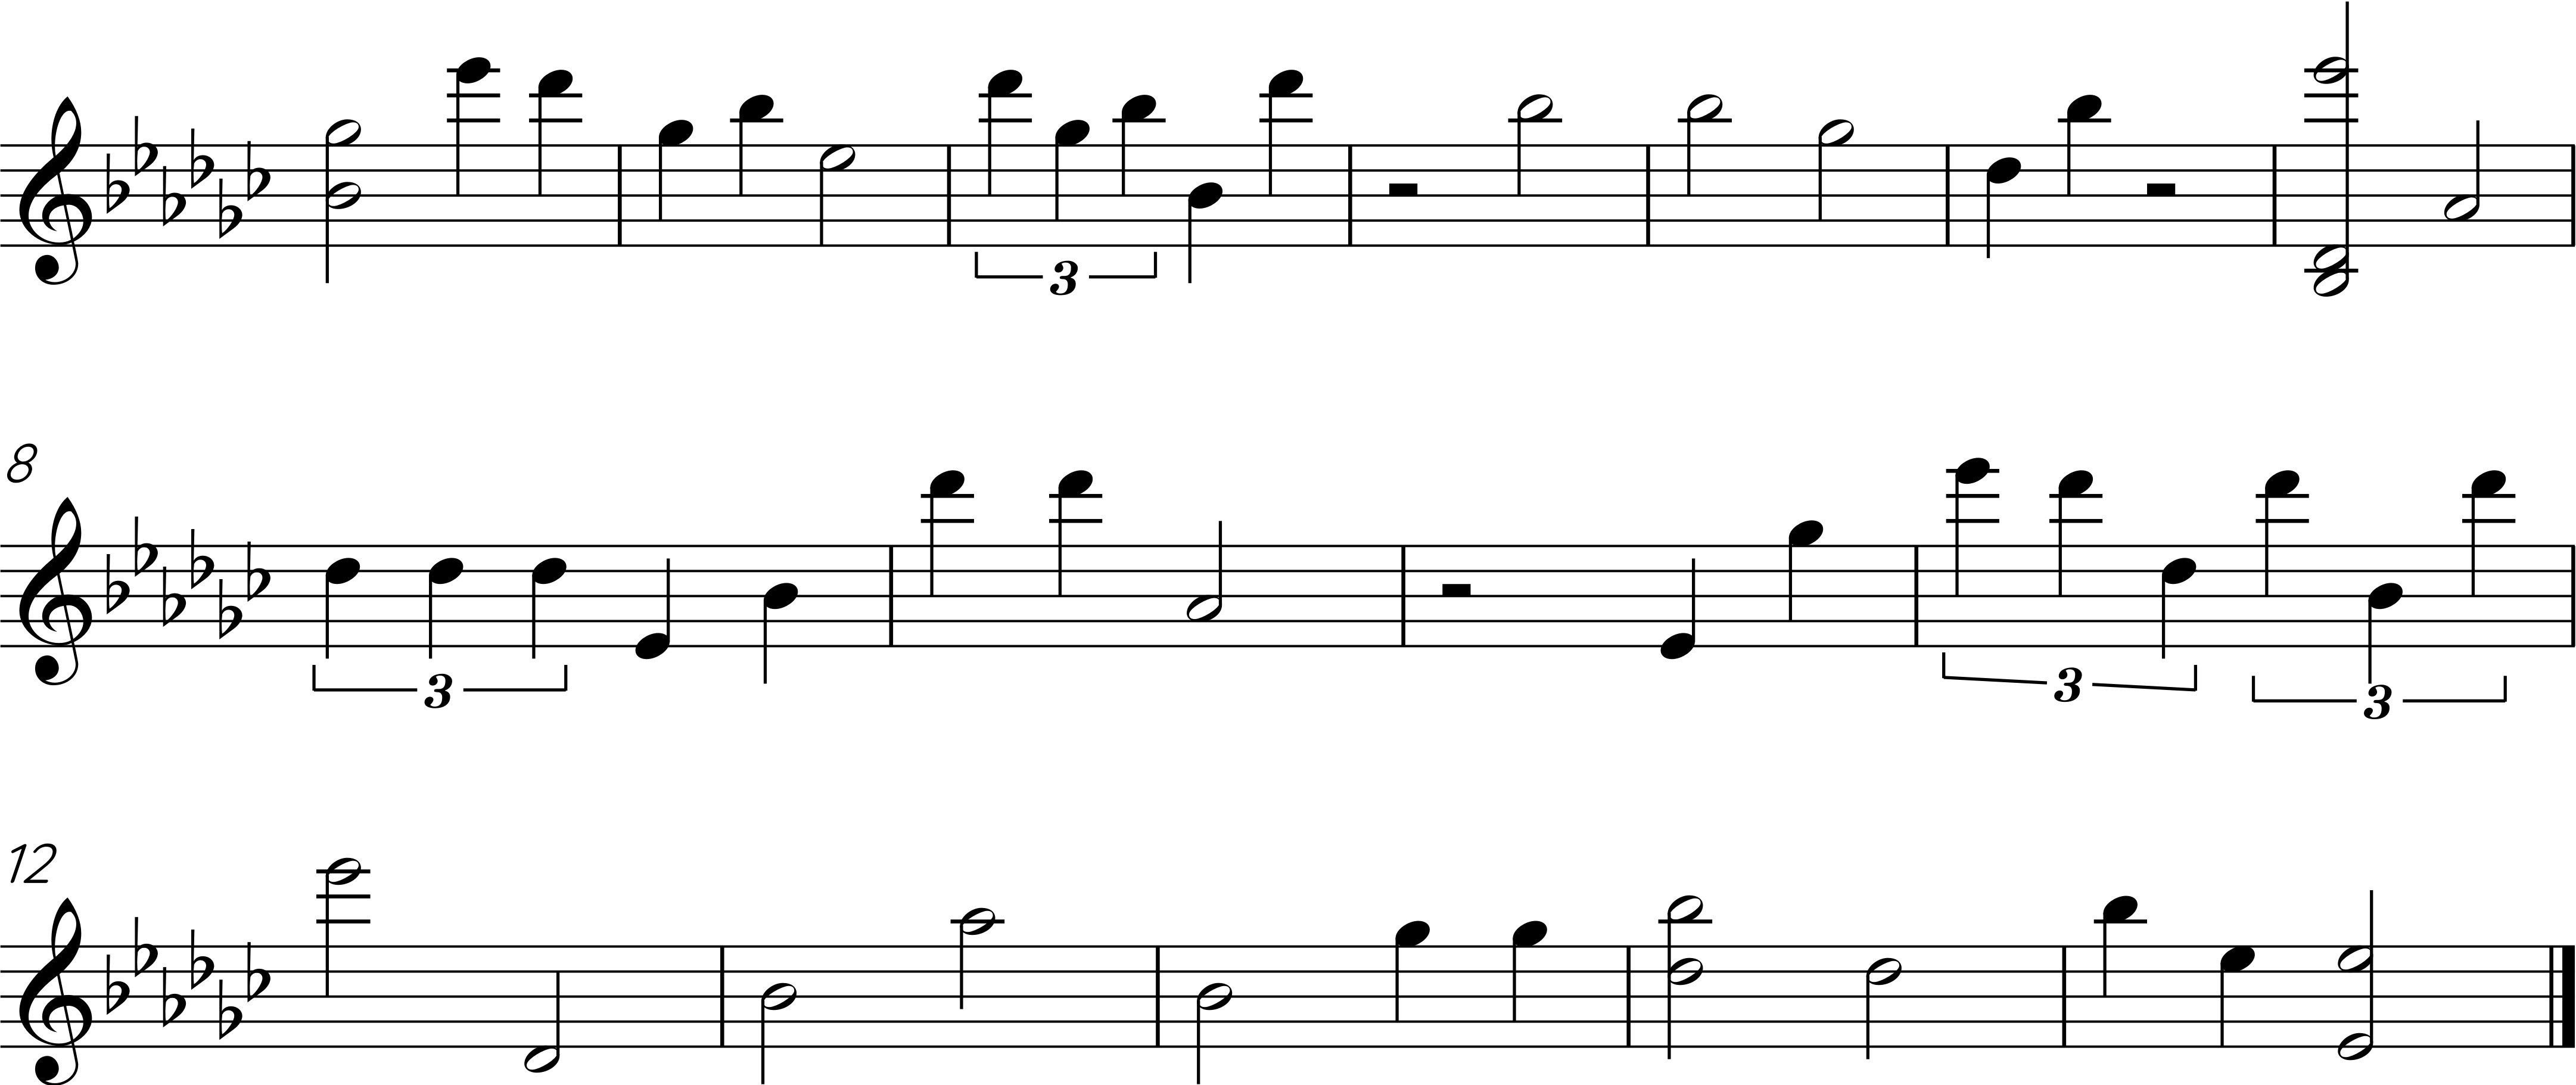
\includegraphics[width=\textwidth]{images/implementation/generated-piano.png}
        \caption{Using the system's algorithm to generate a piano part based on a number of simple cases.}
        \label{fig:generated-piano}
    \end{subfigure}
    ~
    \caption{
    Compared to the \subref{fig:generated-piano-basic} basic algorithm, the \subref{fig:generated-piano} proprietary algorithm creates a much more natural and realistic piano part.
    }\label{fig:piano}
\end{figure}

\subsection{Creating Reactive Instruments}
Not only do the instruments need to sound natural, but their generation should be able to be manipulated by the user. In the piano part, there is a density slider which the user can adjust. By increasing the density, the number which gets inputted into the piano algorithm decreases. This means that there is a higher probability for one of the cases in the switch statement to match, and therefore, a lower probability for the piano not to play at a given timestep. This results in a denser melodic line. This is similar to the marimba instrument’s implementation, where the density decreases the probability of it not playing at a given timestep, and sliding the density to the maximum value leaves the marimba consistently playing a note four times per beat.

The electric guitar instrument, however, has a completely different behaviour from the rest of the instruments in the system. Instead of picking a note or notes to play at a given timestep, the guitar is pre-programmed with a concrete set of MIDI recordings lasting two bars of music each, where each phrase has an associated “intensity” and “density” label. For example, if the user sets the intensity to “medium” and the density to “sparse”, the guitar will randomly pick a pre-recorded phrase which is labelled with medium intensity and sparse density, playing that sample at the start of the next two measures.

The guitar is defined this way to allow for greater expressive control over the instrument, allowing pitch bends, vibrato, and more complex rhythmic phrasing to be included in the samples, which would not be possible if the guitar used the same system as the other instruments.

A downside to this method of implementing the guitar part is that when a user changes a modifier, it will only start playing in the updated parameters after the current two-bar sample finishes playing. This means there is a delay between the user changing the slider and the guitar responding to that change, however, the benefits of greater expressive control were worth this compromise since the rest of the instruments did react immediately to the user’s changes.

Many of the instruments have a “Filter” slider which adjusts the instrument’s filter node, adding either a low or high-pass filter to the instrument. This works by cutting off the frequencies either below or above (depending on the type of filter) a target frequency. By sliding a filter slider to the left, a low-pass filter begins to cut frequencies higher than the slider’s value. Similarly, sliding to the right cuts off frequencies below the target. It is also worth noting that the relationship between pitches and frequencies follows a logarithmic scale, so the linear positions of the filter sliders have to be converted to that scale so that when a user drags the slider linearly, the apparent filter cutoff follows a roughly audibly linear scale.

Adding filters to the instruments can drastically change their tone, with a low-pass filter “muffling” the sound, and a high-pass creating a “tinny” sound when pushed to their respective extents. It was worth adding these so that the user has even more control over the tone of the instruments.

\section{Synchronising with Sockets}
One of the most challenging aspects of this project was ensuring the musical experience was identical across all connected users. This was done by sending and receiving messages through the WebSocket connection. When a user changes a control or modifier in the app, a message is sent to the server indicating which control was changed alongside its updated value. The server forwards all socket messages to any other connected user alongside sending a regular pulse which acts as the music beat.
By making sure every change to the app is sent through to the users in an audio room, the system can ensure consistency across those connected users. This came with additional complexities which had to be resolved for the app to work efficiently and consistently. This section describes some of the technical factors behind creating the finished product.

\subsection{Message Format}
The messages sent through the socket follow a specific format which was developed to efficiently convey system control and state updates. Any message that involves audio includes \verb|type: audio_message| at the beginning of the message to indicate that the app should then parse the rest of the message.

These messages typically contained a \verb|track| field, which indicated which track the change was for. For example, when a user mutes a sequencer sample, the track field would be \verb|sequencer|, or if the user drags an ambience volume slider, the track field would be \verb|ambience|. To parse audio messages, switch statements are used to determine what category of control was made. For each track type, there were subsequent fields such as \verb|target|, \verb|instrument| or \verb|sliderID|.

Audio messages contain a \verb|user| field, which was implemented during testing as when a client sent audio messages to the server, the server would forward that message to all connected users, including the client who sent the message. A result of this was “rubber-banding”, where after making a change to the app, there would be a brief delay before that change was then echoed back to the client and that state update would repeat itself. This was not noticeable with changes such as toggling a track on or off, but when sliding a control slider, the slider would flicker back and forth as it received the client’s own commands while the user was still dragging the slider, typically after <100ms. Fixing this involved sending the username as a field within the socket message. Then, clients could ignore any messages that had their username attached, removing the rubber-banding effect completely.

Instruments, alongside what notes they play, are also triggered by socket messages. Every beat, the server sends messages about the notes that each instrument should play. These can be randomly generated, but since they are generated server-side and then sent to the clients, the random notes are the same notes for each connected user, ensuring a consistent experience.

\subsection{Sending Beats Consistently}
The notes are not the only thing that is required to be consistent, as the rhythm of the music needs to be strictly in time with imperceivable fluctuations in beat consistency. To synchronise the sequencer beats and instrument cues, the server sends beat messages every second, which means the system runs at 60 bpm. This can be thought of as a form of metronome for the clients to play in time with.

At first, the server attempted to send a pulse every 200ms, which at the time was how long each of the 16 sequencer timesteps was supposed to last. This was done by creating an asynchronous server-side worker which sent out the sequencer beat message alongside any instrument cues which would occur on that timestep, then slept for 200ms. When running the server locally this worked fairly consistently, however, once deployed, the latency was very inconsistent and beats would regularly arrive late.

After experimenting with different sleep durations, it was apparent that regardless of the sleep duration, there was ~200ms additional latency which when built up over the 16 timesteps added up to over 3 seconds of average unintended delay. Additionally, the total duration of a bar of music would last anywhere between 5100 and 6600ms. This was obvious when using the sequencer, as beats would drastically slow down and speed up over time.

To fix this, the server should no longer rely on sleeping after sending socket messages, and it was apparent that the time taken to send those socket messages would vary by a large margin. The solution was to reduce the amount of socket messages by over 80\% and instead send one pulse every 1000ms rather than every 200ms. This pulse would also not depend on how long the previous task took but instead use the server’s very accurate system time to measure the time until the next system second, then delay by that amount.

By doing this, the average bar duration variance fell from over 1500ms to <25ms, an approximately 98\% reduction. This led to an audible improvement in beat consistency, as beats would arrive with imperceptibly small fluctuations, with most of these due to the internet connection with the remote server, which is located in London.

Reducing the server’s update frequency from 4 updates per beat to 1 resulted in a major refactoring to the socket format, particularly to the sequencer. Previously, the server would send 16 updates per bar which directly triggered the sequencer to play one of its timesteps. After the change, clients receive one server beat update every four sequencer timesteps. Because of this, when a server beat message is received by the client (every 1000ms), it plays the first of the timestep of the beat instantly, then sets three internal timeouts: 250, 500, and 750ms respectively, where each of these timeouts plays one of the other subsequent sequencer timesteps. For example, when the client receives “Beat 1”, the sequencer plays timestep 0, waits 250ms, plays timestep 1, waits, plays 2, waits, and plays 3. Then in 250ms time, the client should expect to receive “Beat 2” from the socket which triggers sequencer timesteps 4-7.

By combining occasional but accurate server pulses with local timeouts, the user experiences a very consistent rhythm which is important for the immersive aspect of the app.

\section{Deployment}

Hosting the app on a live remote server where it can be publicly accessed was a key part of this project. Through the deployment stage, the collaborative aspects of the system could be tested and optimised in a real-world context with real-world latency and network limitations, rather than hosting the server on a local network where latency is negligible.

\subsection{Preparing for Deployment}
The system had to incorporate several changes to be ready for deployment. First, static files such as images, scripts, stylesheets and audio samples had to be served through the server rather than Django. Then, a remote Redis server had to be set up and linked to act as a storage layer and to dispatch the WebSocket messages. Additionally, a population script was created so that whenever the app was deployed onto the remote server the rooms would be correctly set up.

\subsection{Network Optimisation}
As discussed previously, the beat update messages which triggered the sequencer beats and cued instruments to play underwent significant changes after deploying and testing on the remote site. This was not the only change which was required to make the system usable, and various network optimisation techniques were used to streamline the experience.

Most of the slider controls on the site use a range between 0 and 200. These sliders use event listener functions which wait for user input before executing a function, usually consisting of altering the local sound of the system, then sending a socket message to synchronise the other users in the room. Because these listeners trigger on every input, if a user sliders a slider from its minimum to the maximum value, there are 200 events in a fairly short period (depending on how fast the user drags the slider). At first, the event listener function sent a socket message on every single input, which meant that hundreds of messages would be sent through the socket when a user changed a slider value. During testing, this caused a significant slow-down, as the server could not keep up with sending up to hundreds of messages a second.

\subsection{Reducing Message Frequency}
To fix this issue, the event listener only sends a socket message periodically instead of on every single input, in many cases when the slider value is a multiple of 5 or 10. Instead of sending 200 messages for a min-max slider drag, the client only sends 40 or 20 respectively. Of course, this meant that the other users would only receive a quantised value, to the nearest 5 or 10. For example, if user 1 drags a slider to 68, the socket’s most recent message would tell user 2 to set the value to 65. To maintain the accuracy of the synchronisation, a new event listener was added which waited for the “hover off” event. Then, when a user’s mouse cursor leaves the slider, the final precise value is sent through the socket.

By implementing the updates in this way, the socket message frequency and therefore server load is decreased, while the accuracy of the synchronisation is maintained.


\chapter{Evaluation} 
% How good is your solution? How well did you solve the general problem, and what evidence do you have to support that?
% Ask specific questions that address the general problem.
% Answer them with precise evidence (graphs, numbers, statistical analysis, qualitative analysis).
% Be fair and be scientific.
% The key thing is to show that you know how to evaluate your work, not that your work is the most amazing product ever.

To evaluate the system and assess how successfully it meets the requirement specification, a user evaluation was conducted. First, there were tasks for the user to complete, then a survey on their experience.

\section{Participants}
It was important to obtain participants with a variety of backgrounds, particularly in musical experience. While the app may be intuitive to users with experience in music production due to the skeuomorphic design (as discussed in the design chapter), it was crucial to understand how users with little or no music-making experience would navigate and use the systems. With the goal of creating an accessible, engaging, and intuitive app, analysing participants with a range of prior musical experiences would be crucial in determining the success of the project.

\section{Format}
First, participants performed two tasks: One was an individual exercise where they used the system by themselves, following the structure of a typical session by adding tracks one by one to create a final mix. Then, the participant was instructed to repeat a similar exercise but instead with another user connected to the audio room. The full task handout is available in Appendix \ref{appendix:handout}.

After performing the two tasks, a user survey was filled out. This asked questions about the participant’s musical experience, engagement and enjoyment of the app and whether the systems allowed for sufficient control. After this, there were some open-ended questions in which participants could provide feedback on the system, including suggestions on improvements of features they would like to see implemented on the app. The full user survey is available in Appendix \ref{appendix:questions}.

\section{Results}
The survey was primarily qualitative, with most questions answered using a five-point Likert scale. The full results can be found in Appendix \ref{appendix:responses}. All participants responded positively to the experience, agreeing that the system was enjoyable, immersive, relaxing, and engaging. Additionally, participants enjoyed using the app more with another person, and results showed that they were more engaged, although the collaborative experience was less relaxing compared to using the app individually. Participants also generally felt a social connection to the other user while using the app, which was a crucial aspect of the requirements of the project.

It was also clear that regardless of musical experience, participants could understand and feel immersed in the music-making process. They also enjoyed the simplicity of the controls, although participants with more music-making experience were more likely to suggest more control or more instruments/samples. This makes sense because if participants already had experience with contemporary music production software like DAWs, they may feel that the app had a limited set of controls in comparison.

All participants were able to figure out what the controls of the various panels did. The only confusing control was the filter, which applied a low or high-pass cutoff on the associated sound. This was especially confusing for participants with no music production experience, as, despite the app showing what cutoff frequency was active, they needed to understand what the frequency represented or how it related to the sound. However, participants who were confused later noted that once they started using the slider, they could hear the difference in sound.

\section{Suggestions}
Participants were given an opportunity to suggest new features or changes to the app. Generally, they were happy with the state of the site, however, some participants suggested features such as being able to change the tempo of the music or more effects added to the instruments. More freedom with the instruments was a common theme among suggestions and this is a point worth considering for future work.

The interface was unanimously received as easy to use and pleasing to look at. The only problems were with users with smaller displays, in which elements would sometimes overlap or not display correctly. This was corrected in a later version of the site by adding media queries and changing the position of certain elements based on the site of the user’s screen.

\section{Summary}
Overall, the user evaluation was successful in identifying key aspects which participants focused on as well as in understanding how successful the social and musical features were. There was useful feedback which allowed for further development into the user experience, as well as insightful information on how participants felt during both the individual and collaborative exercise. The evaluation also proves the project meets the requirements defined in the requirements specification.

\chapter{Conclusion}    
Summarise the whole project for a lazy reader who didn't read the rest (e.g. a prize-awarding committee). This chapter should be short in most dissertations; maybe one to three pages.
\section{Guidance}
\begin{itemize}
    \item
        Summarise briefly and fairly.
    \item
        You should be addressing the general problem you introduced in the
        Introduction.        
    \item
        Include summary of concrete results (``the new compiler ran 2x
        faster'')
    \item
        Indicate what future work could be done, but remember: \textbf{you
        won't get credit for things you haven't done}.
\end{itemize}

\section{Summary}
Summarise what you did; answer the general questions you asked in the introduction. What did you achieve? Briefly describe what was built and summarise the evaluation results.

\section{Reflection}
Discuss what went well and what didn't and how you would do things differently if you did this project again.

\section{Future work}
Discuss what you would do if you could take this further -- where would the interesting directions to go next be? (e.g. you got another year to work on it, or you started a company to work on this, or you pursued a PhD on this topic)

\begin{appendices}

\chapter{Evaluation Handout}\label{appendix:handout}
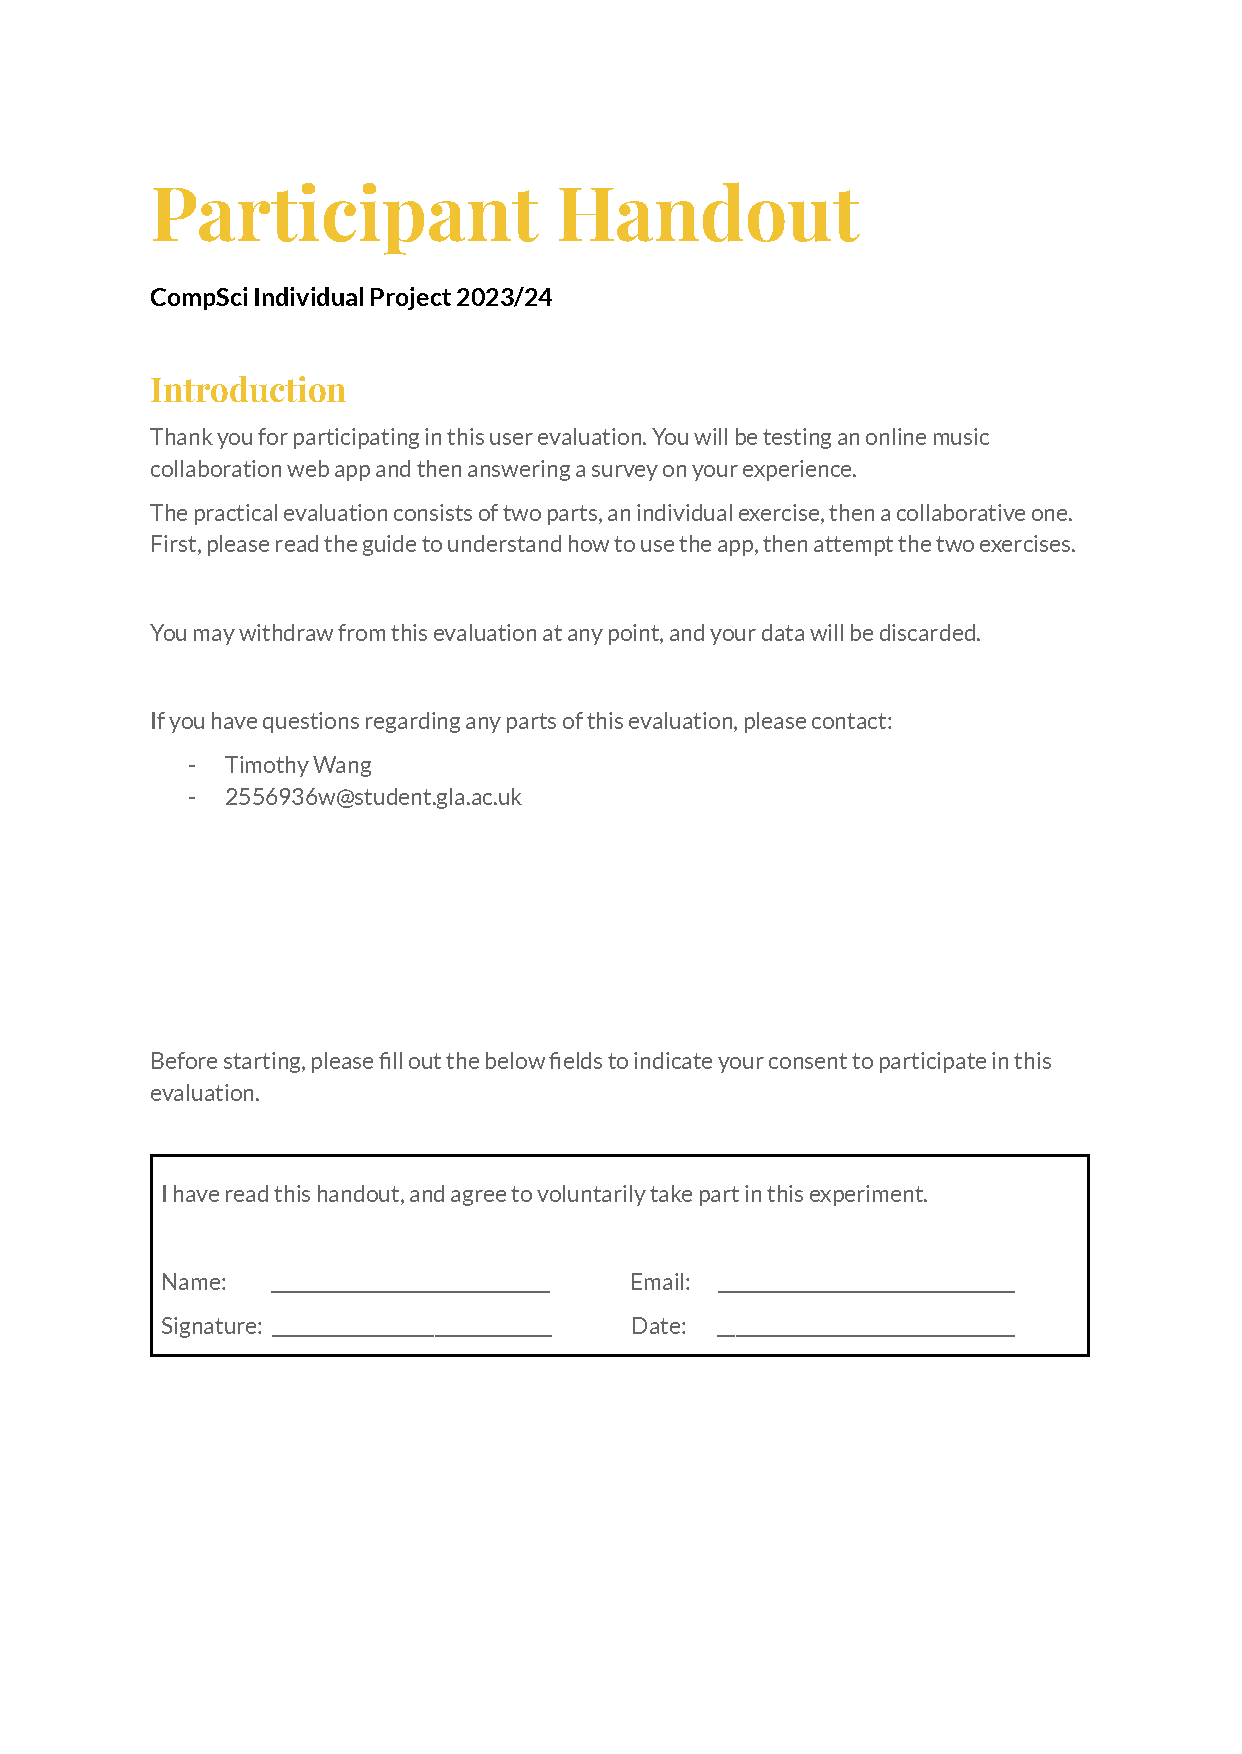
\includepdf[pages=-,pagecommand=\thispagestyle{plain}]{appendices/evaluation-handout.pdf}

\chapter{User Survey Questions}\label{appendix:questions}
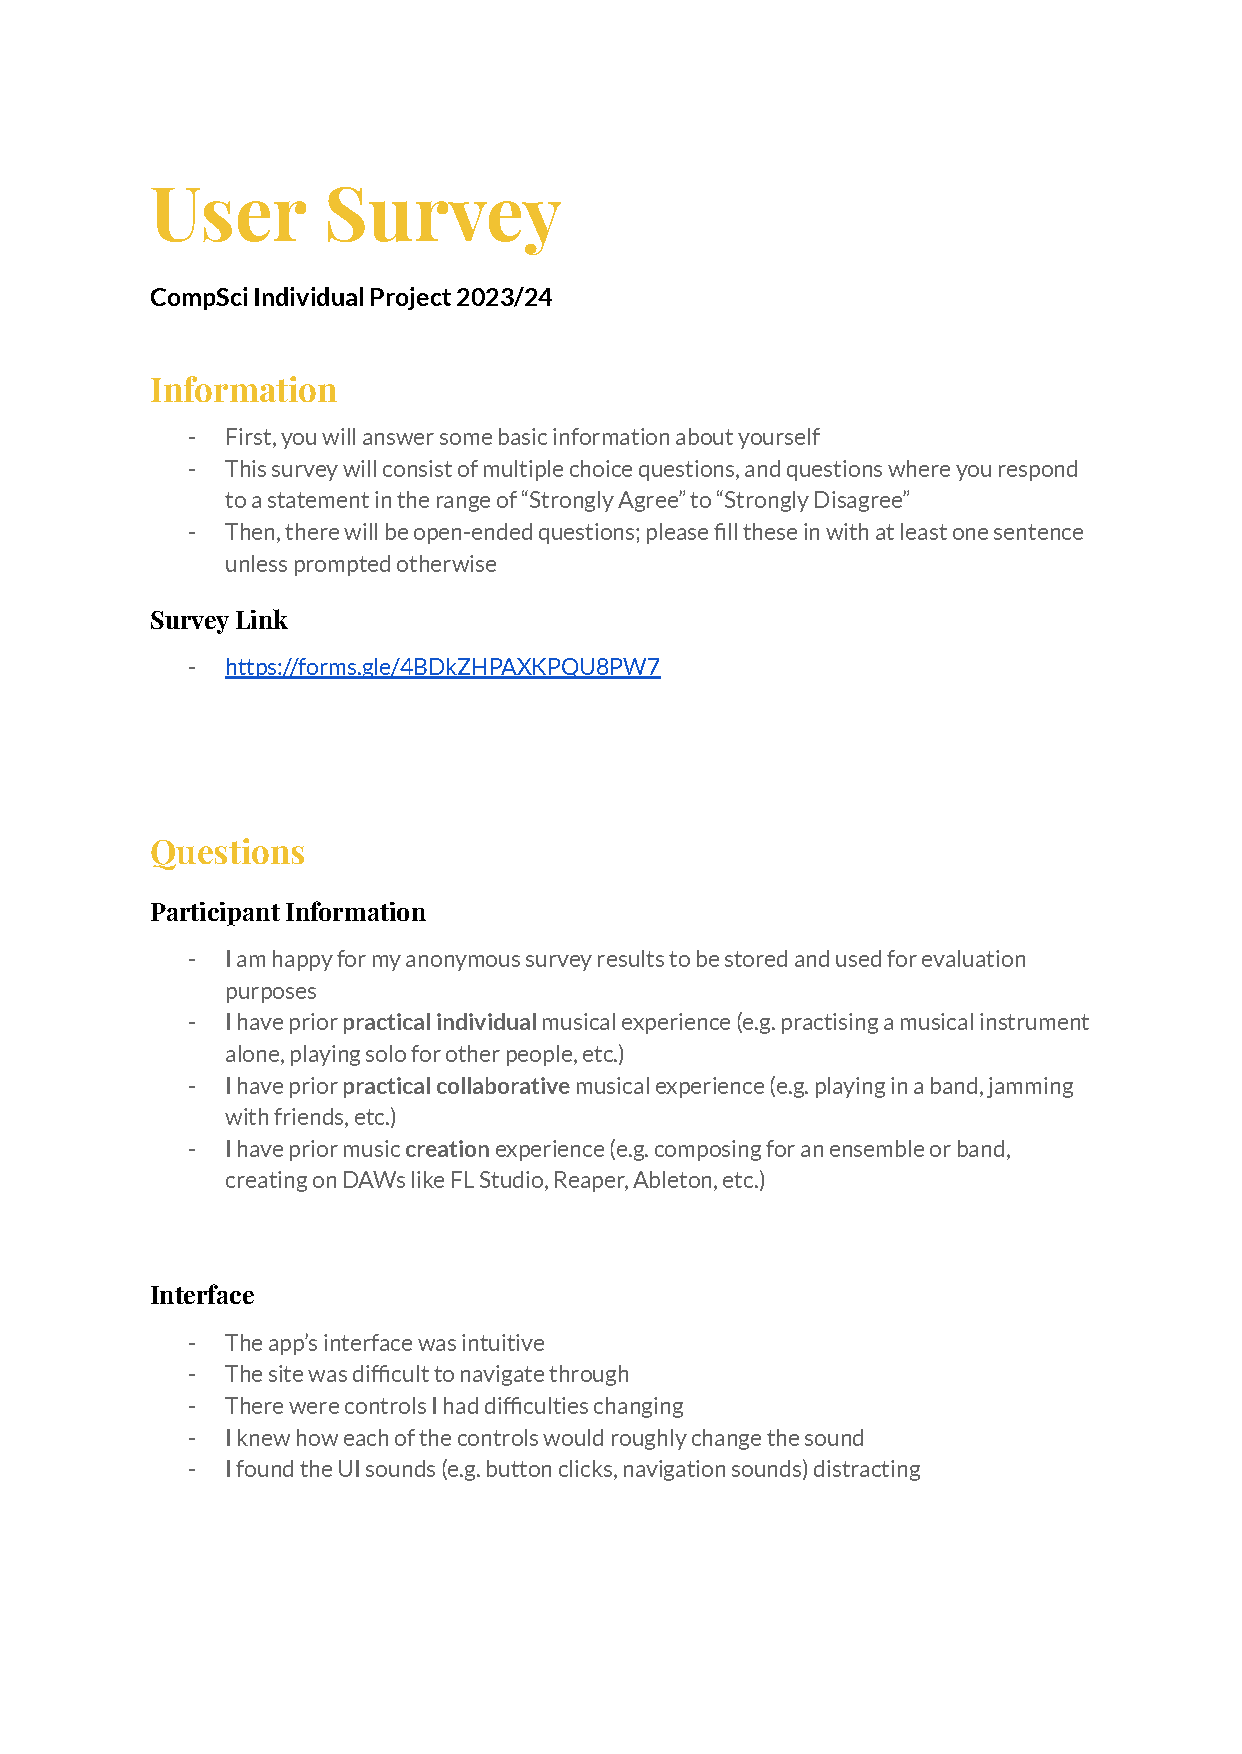
\includepdf[pages=-,pagecommand=\thispagestyle{plain}]{appendices/user-survey.pdf}

\chapter{Survey Reponses}\label{appendix:responses}

\begin{figure}[htb]
    \centering
    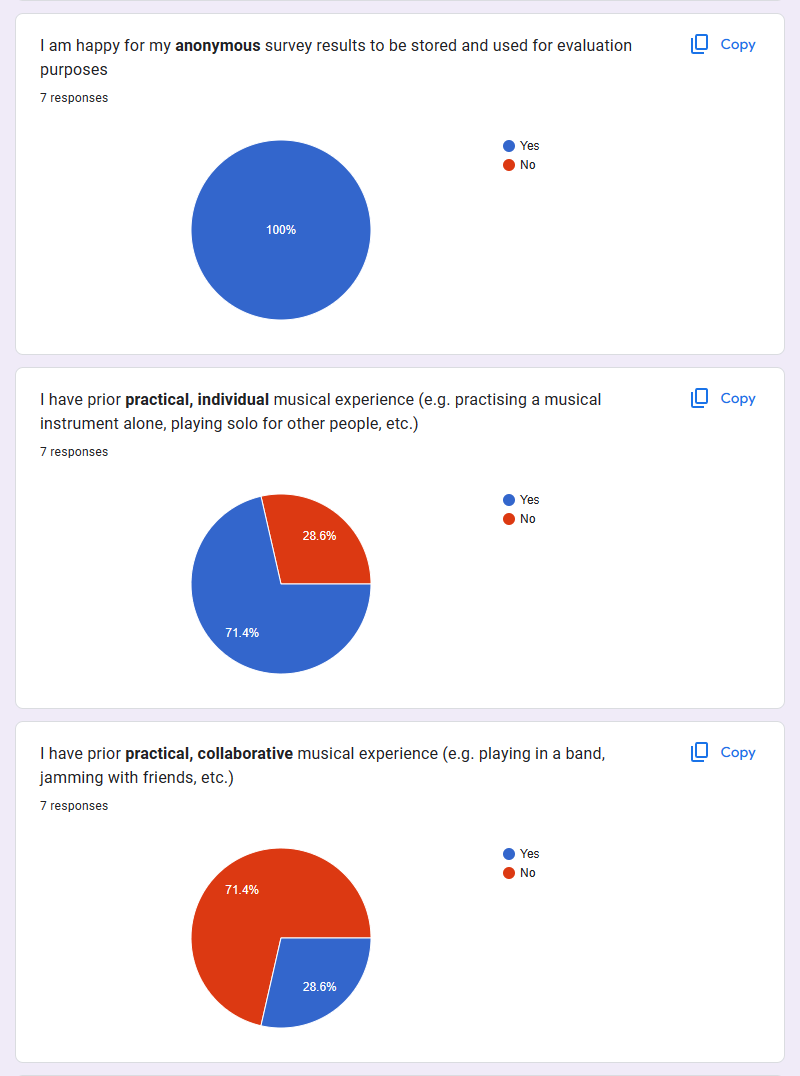
\includegraphics[width=0.8\linewidth]{images/survey-results/1.png}    
\end{figure}
\begin{figure}[htb]
    \centering
    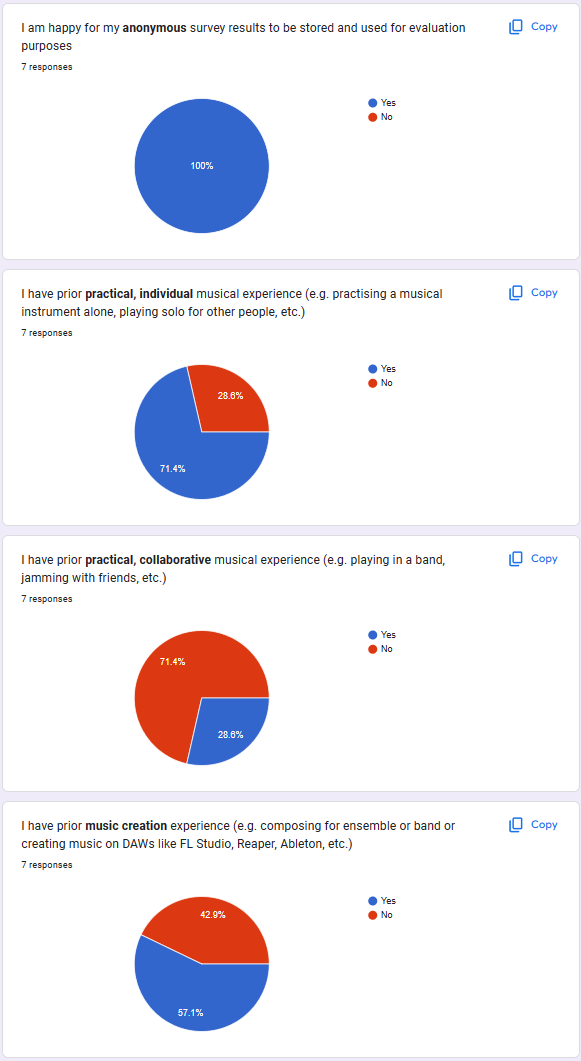
\includegraphics[width=0.8\linewidth]{images/survey-results/2.png}    
\end{figure}
\begin{figure}[htb]
    \centering
    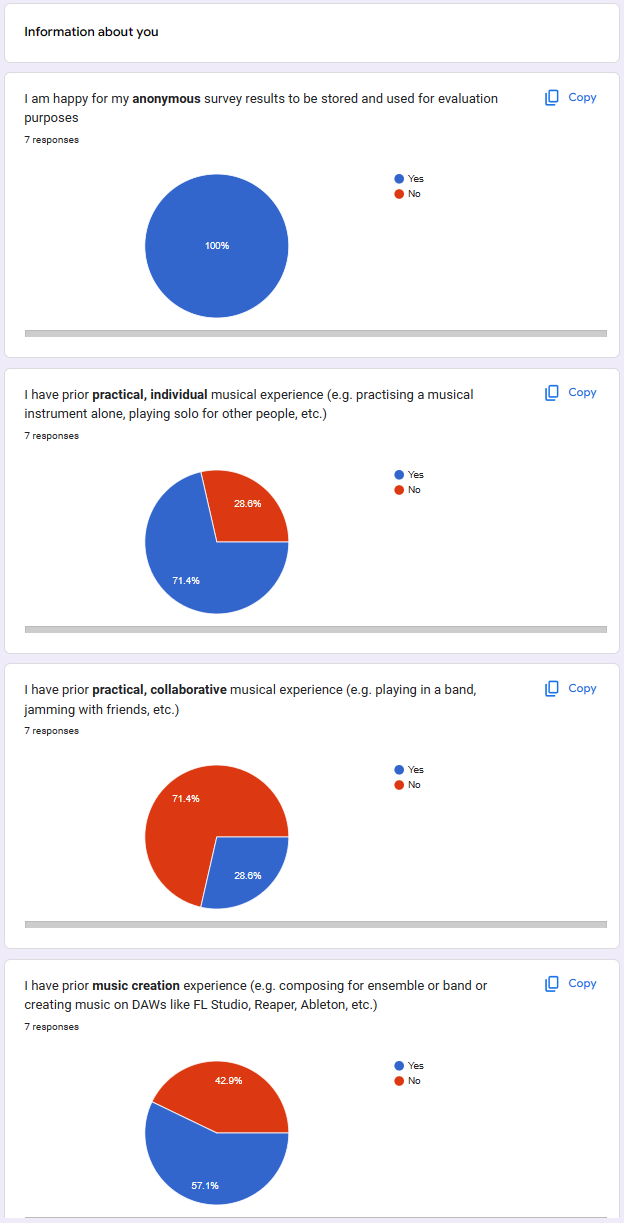
\includegraphics[width=0.8\linewidth]{images/survey-results/3.png}    
\end{figure}
\begin{figure}[htb]
    \centering
    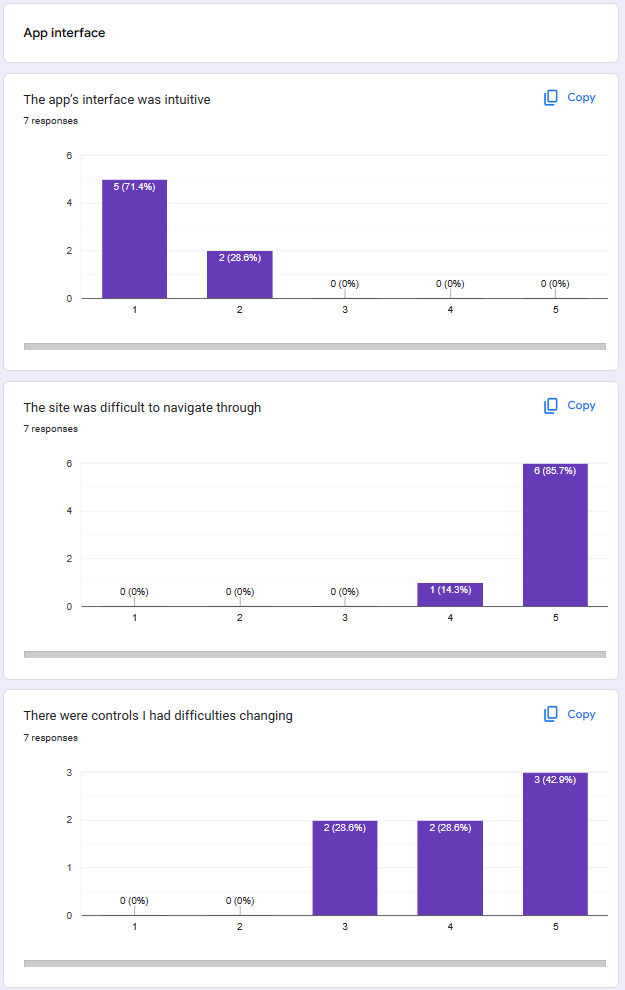
\includegraphics[width=0.8\linewidth]{images/survey-results/4.png}    
\end{figure}
\begin{figure}[htb]
    \centering
    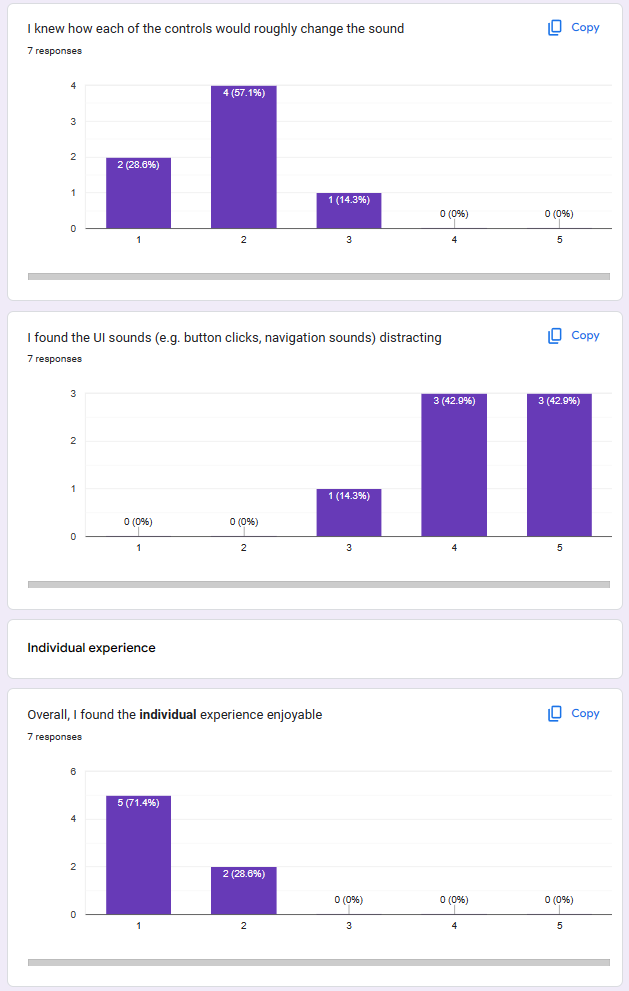
\includegraphics[width=0.8\linewidth]{images/survey-results/5.png}    
\end{figure}
\begin{figure}[htb]
    \centering
    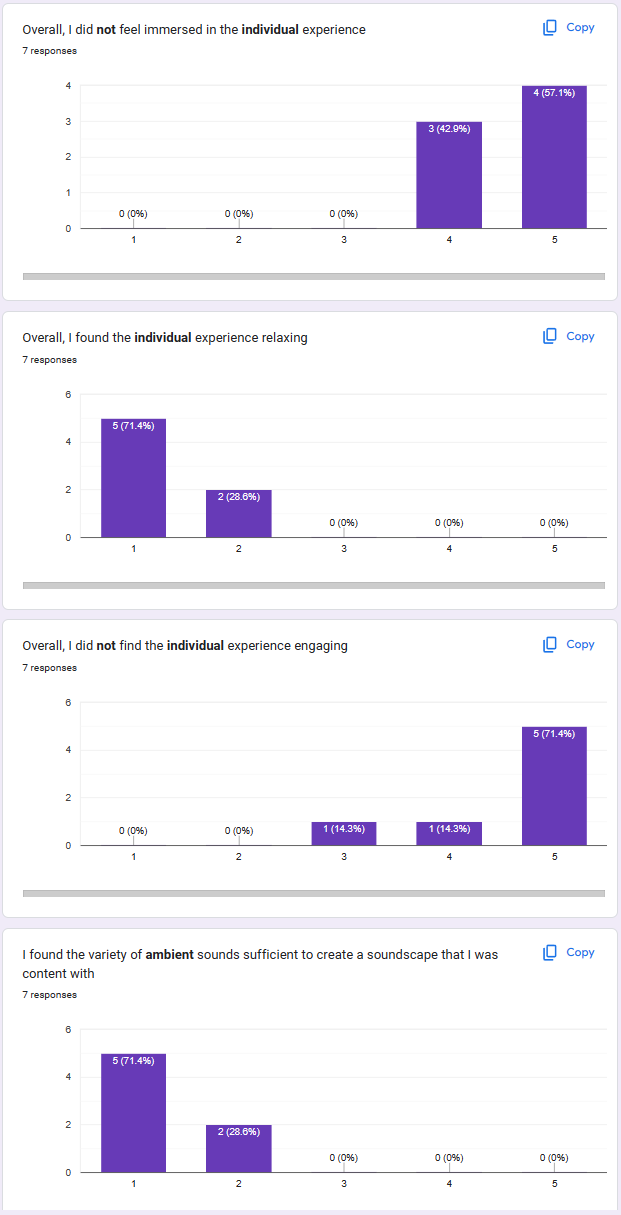
\includegraphics[width=0.8\linewidth]{images/survey-results/6.png}    
\end{figure}
\begin{figure}[htb]
    \centering
    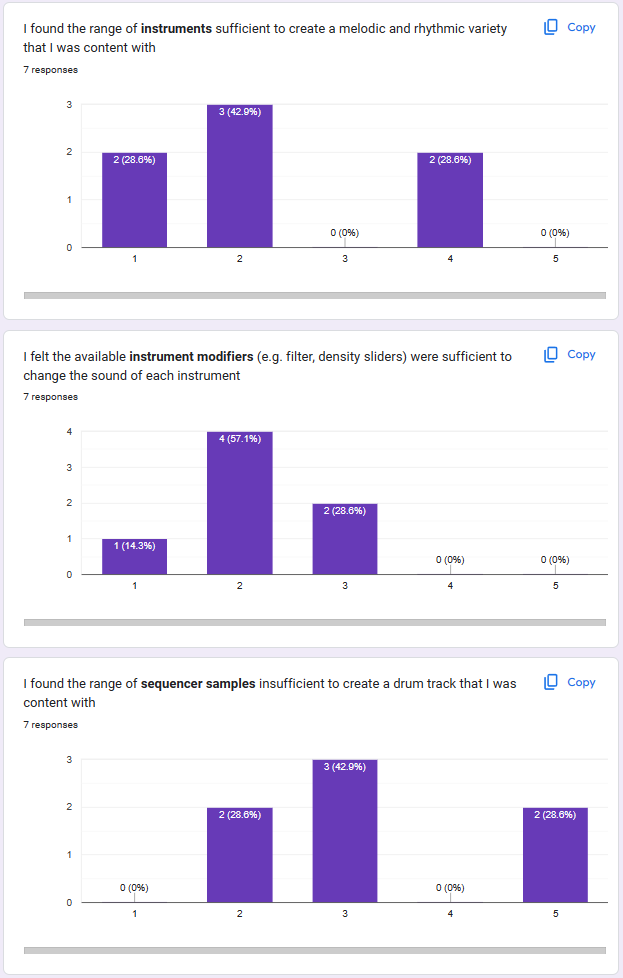
\includegraphics[width=0.8\linewidth]{images/survey-results/7.png}    
\end{figure}
\begin{figure}[htb]
    \centering
    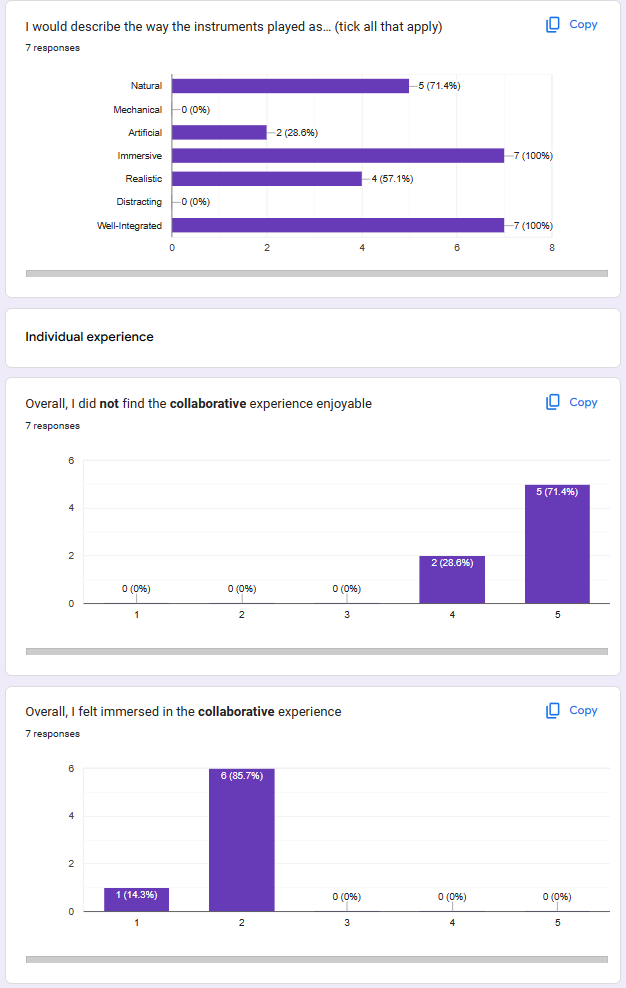
\includegraphics[width=0.8\linewidth]{images/survey-results/8.png}    
\end{figure}
\begin{figure}[htb]
    \centering
    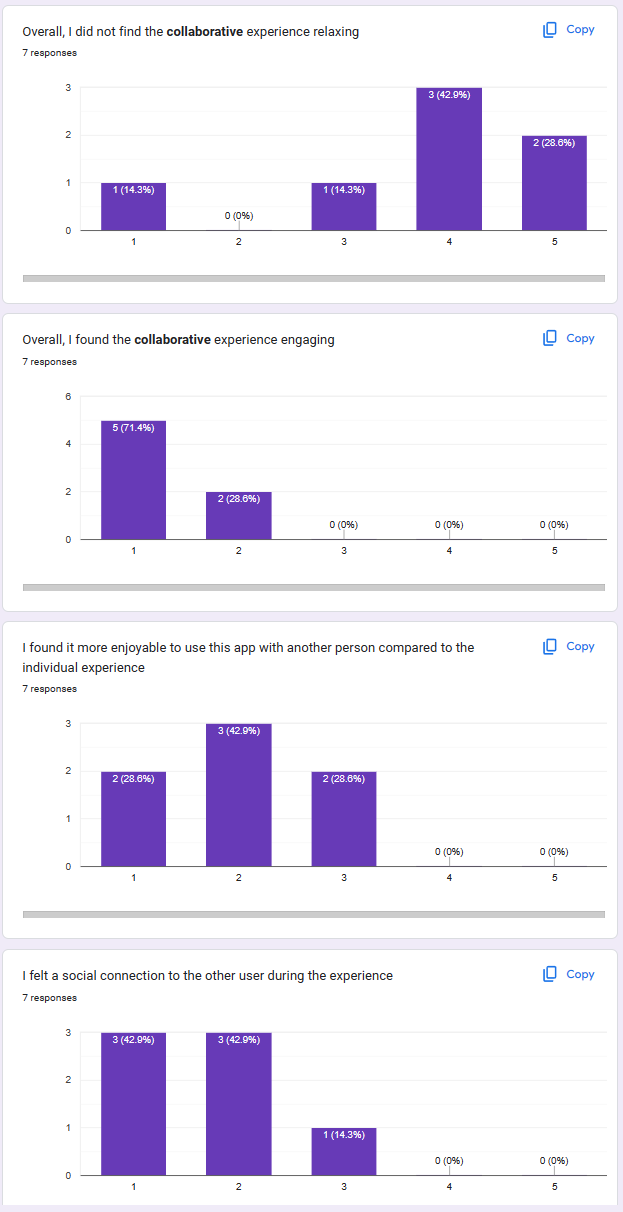
\includegraphics[width=0.8\linewidth]{images/survey-results/9.png}    
\end{figure}
\begin{figure}[htb]
    \centering
    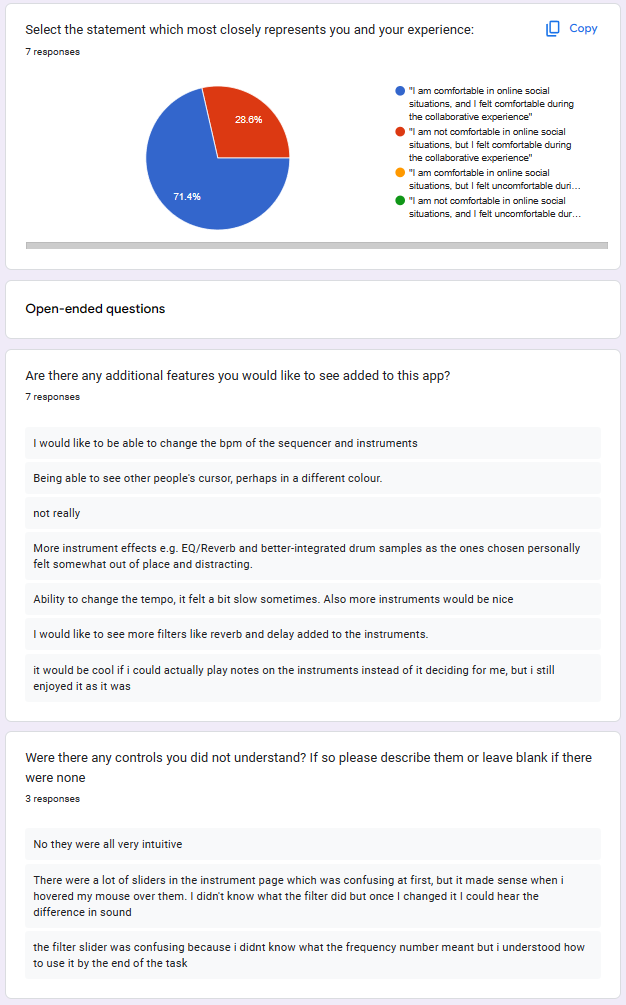
\includegraphics[width=0.8\linewidth]{images/survey-results/10.png}    
\end{figure}\begin{figure}[htb]
    \centering
    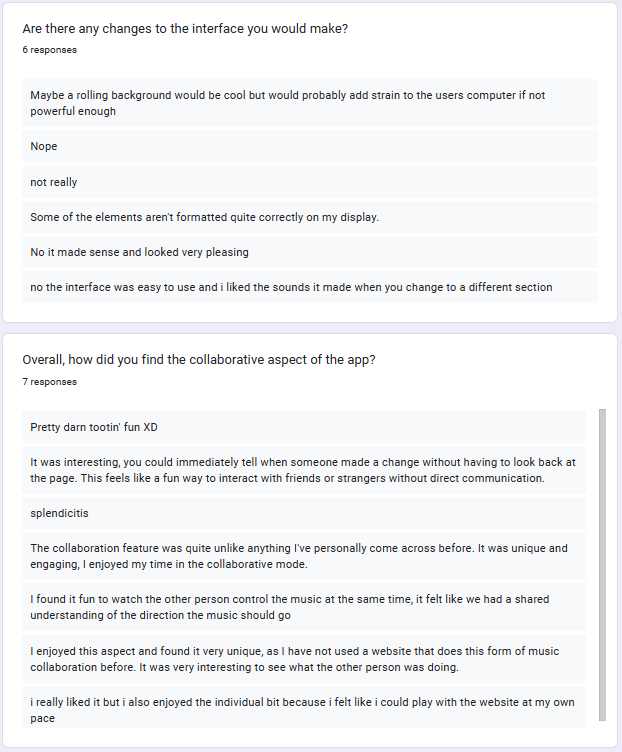
\includegraphics[width=0.8\linewidth]{images/survey-results/11.png}    
\end{figure}

\chapter{Ethics Form}\label{appendix:ethics}
(Document is signed and dated but may not appear so. Open the document separately if this is the case.)
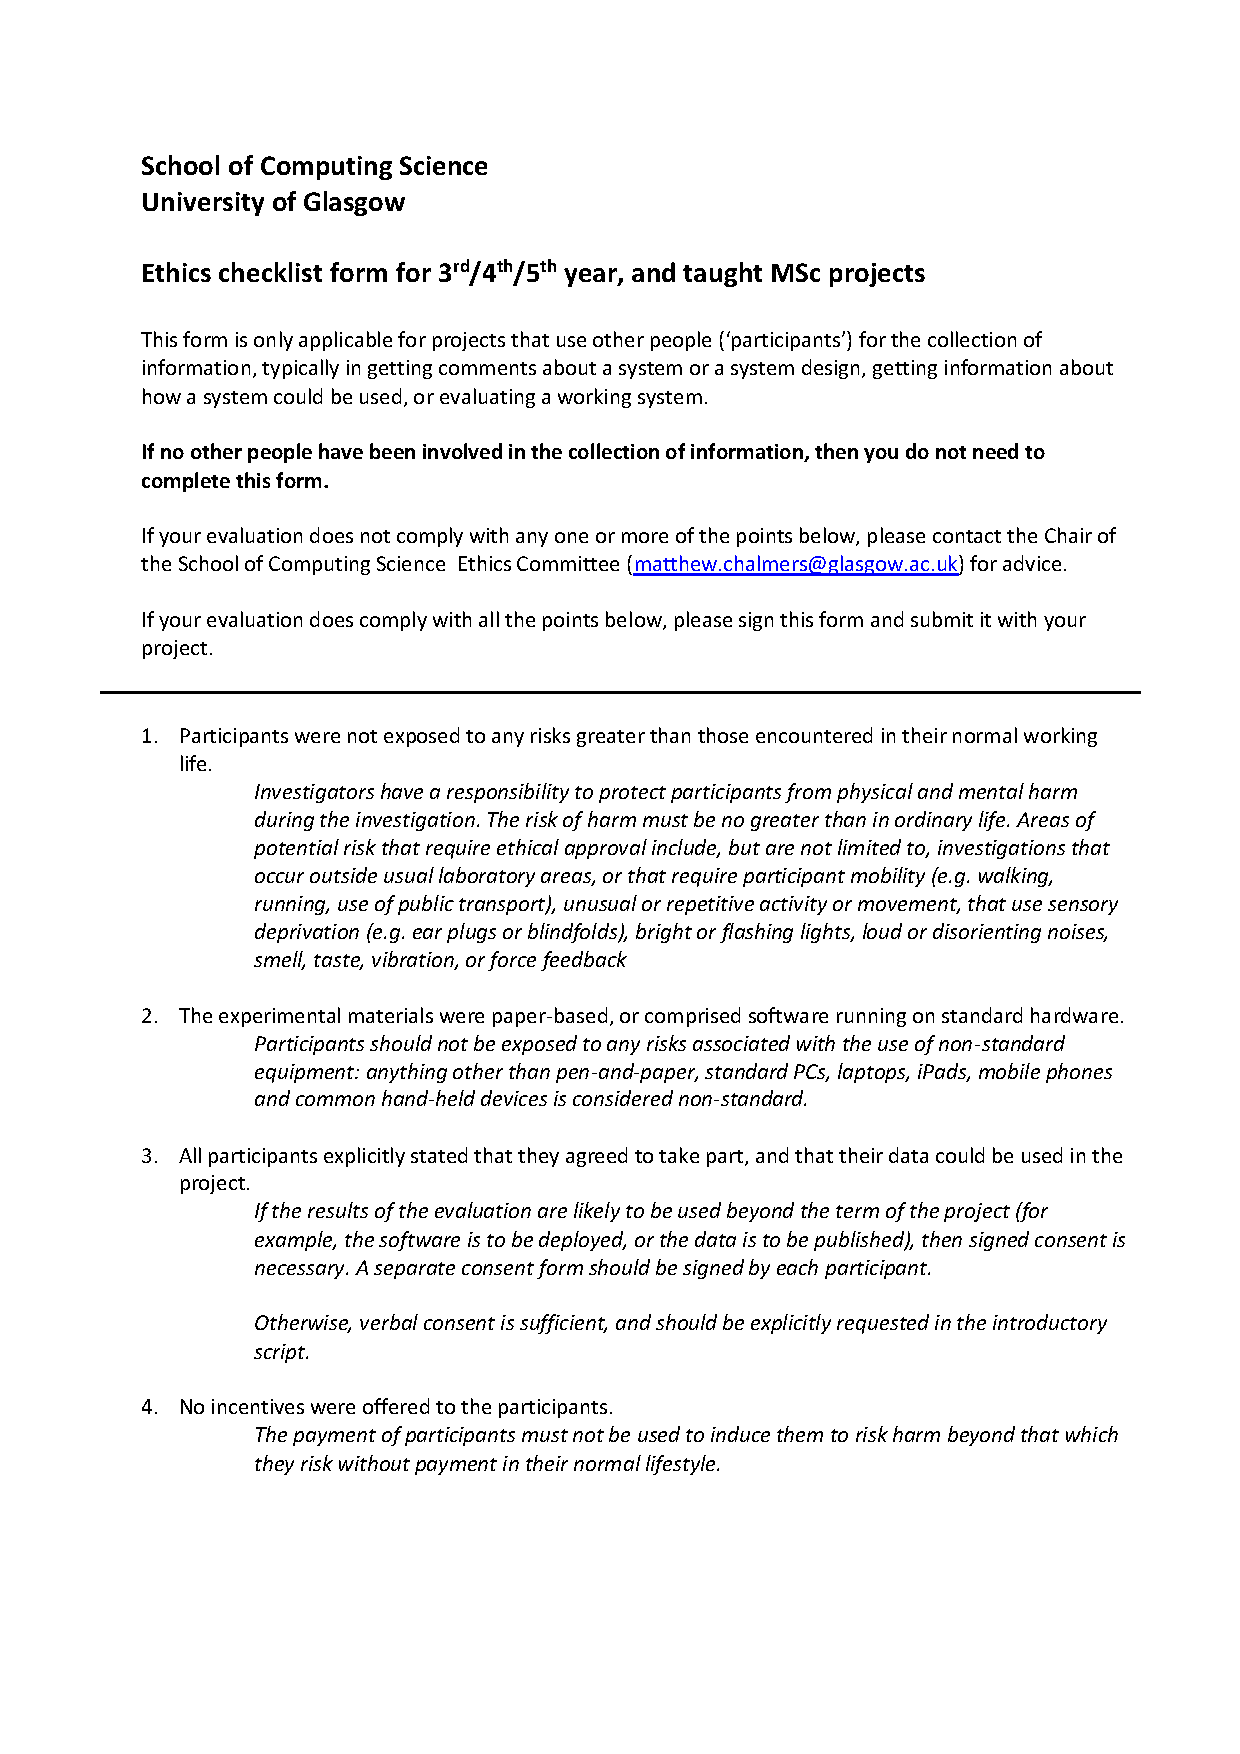
\includepdf[pages=-,pagecommand=\thispagestyle{plain}]{appendices/ethics-form.pdf}

\end{appendices}

% The bibliography style is agsm (Harvard)
% The bibliography always appears last, after the appendices.

\bibliographystyle{agsm}

% Force the bibliography not to be numbered
\renewcommand{\thechapter}{0} 
\bibliography{l4proj}

%==================================================================================================================================

\end{document}
